\documentclass[11pt,a4paper]{article}
\usepackage{amsmath}
\usepackage{amsthm}
\usepackage{graphicx}
\usepackage[linesnumbered, ruled, vlined]{algorithm2e}
\usepackage[noend]{algpseudocode}
\usepackage{enumerate}
\usepackage{xcolor}
\usepackage{framed}
\usepackage{bm}
\usepackage{pifont}
\usepackage{multicol}
\usepackage{lipsum}
\usepackage{tikz}
\usetikzlibrary{calc}
\usepackage{array}
\usepackage{relsize}
\usepackage{comment}
\usepackage{url}
\usepackage{caption}
\usepackage{subcaption}
\usepackage{mathtools}
\usepackage{thmtools}
\usepackage{thm-restate}
\usepackage[normalem]{ulem}
\usepackage{cleveref}
\usepackage{xspace}
\usepackage{amssymb}
% ======================================================================
% Editing / collaboration
% ======================================================================

% Show diff (exactly one of this and the following pair of commands must be commented)
\newcommand{\add}[1]{\textcolor{blue}{#1}}
\newcommand{\del}[1]{\textcolor{gray}{#1}}

% Preview changes (exactly one of this and the previous pair of commands must be commented)
% \newcommand{\add}[1]{#1}
% \newcommand{\del}[1]{}

\newcommand{\replace}[2]{\del{#1}\add{#2}}

% Enable rendering of comments
% \newcommand{\guy}[1]{[\textcolor{blue}{\textbf{gg:}} {\footnotesize
% \textcolor{purple}{#1}]}}
% \newcommand{\matej}[1]{[\textcolor{blue}{\textbf{mp:}} {\footnotesize
% \textcolor{teal}{#1}]}}
% \newcommand{\marko}[1]{[\textcolor{blue}{\textbf{mv:}} {\footnotesize
% \textcolor{purple}{#1}]}}
% \newcommand{\arp}[1]{[\textcolor{blue}{\textbf{arp:}} {\footnotesize
% \textcolor{brown}{#1}]}}
% \newcommand{\jorge}[1]{[\textcolor{blue}{\textbf{js:}} {\footnotesize
% \textcolor{violet}{#1}]}}
% \newcommand{\akosh}[1]{[\textcolor{blue}{\textbf{af:}} {\footnotesize
% \textcolor{blue}{#1}]}}
% \newcommand{\cmt}[1]{[\textcolor{blue}{\textbf{CMT:}} {\footnotesize
% \textcolor{red}{#1}]}}
% \newcommand{\TODO}[1]{[{\textbf{\red{TODO:}}} {\footnotesize
% \textcolor{gray}{#1}]}}

% Disable rendering of comments.
\newcommand{\guy}[1]{}
\newcommand{\matej}[1]{}
\newcommand{\marko}[1]{}
\newcommand{\arp}[1]{}
\newcommand{\jorge}[1]{}
\newcommand{\akosh}[1]{}
\newcommand{\cmt}[1]{}
\newcommand{\TODO}[1]{}

\newcommand{\ignore}[1]{}

% ======================================================================
% Formatting macros
% ======================================================================

% Some text colors
\newcommand{\blue}[1]{{\color{blue}{#1}}}
\newcommand{\red}[1]{{\color{red}{#1}}}
\newcommand{\out}[1]{{\red{\sout{#1}}}}

\newcommand{\subnetName}[1]{\textbf{\texttt{#1}}}
\newcommand{\actorName}[1]{\texttt{#1}}
\newcommand{\dataField}[1]{\texttt{#1}}
\newcommand{\funcName}[1]{\textit{\texttt{#1}}}
\newcommand{\funcParam}[1]{\textit{#1}}
\newcommand{\accountName}[1]{\texttt{#1}}
\newcommand{\accountNameFull}[2]{\subnetName{#1}.\texttt{#2}}
\newcommand{\tx}[1]{\textit{#1}}
\newcommand{\funcNameFull}[3]{\subnetName{#1}.\actorName{#2}.\funcName{#3}}
\newcommand{\var}[1]{\textit{#1}}

\newtheorem{example}{Example}

% ======================================================================
% Macros for names to use in the text
% ======================================================================

\newcommand{\ipcFull}{Interplanetary Consensus\xspace}
\newcommand{\ipc}{IPC\xspace}
\newcommand{\sa}{\actorName{ISA}\xspace}
\newcommand{\saOf}[1]{$\sa_\subnetName{#1}$}
\newcommand{\saFull}{IPC Subnet Actor\xspace}
\newcommand{\saFulls}{IPC Subnet Actors\xspace}
\newcommand{\gw}{\actorName{IGA}\xspace}
\newcommand{\gwFull}{IPC Gateway Actor\xspace}
\newcommand{\actor}{actor\xspace} % TODO: Get rid of these and use the word "actor" directly in text. The name is very unlikely to change.
\newcommand{\actors}{actors\xspace}
\newcommand{\pofFull}{Proof of Finality\xspace}
\newcommand{\pofsFull}{Proofs of Finality\xspace}
\newcommand{\pof}{\textit{PoF}\xspace}
\newcommand{\postoffice}{postbox\xspace}

% ======================================================================
% Legacy macros
% ======================================================================

\newtheorem{claim}{Claim}
\newtheorem{notation}{Notation}
\newtheorem{invariant}{Invariant}
\newtheorem{execution}{Execution}
\newtheorem{ensemble}{Ensemble}
\newtheorem*{ensemble*}{Ensemble}
\newtheorem{strategy}{Strategy}
\newtheorem*{strategy*}{Strategy}
\newtheorem{assumption}{Assumption}
\newtheorem*{theorem*}{Theorem}

\newcommand{\alg}{$\mathcal A$}
\newcommand{\act}{\alpha}
\newcommand{\wrt}{w.r.t.\/}
\newcommand{\adv}{\sigma}
\newcommand{\SN}{\mathcal{SN}}
\newcommand{\PN}{\mathcal{PN}}
\newcommand{\parent}[1]{\texttt{parent}(#1)}
\newcommand{\user}{u}
\newcommand{\fil}{\textit{amt}\xspace}
\newcommand{\txwf}{$tx(\fil,\; \user,\; fee)$\xspace} %tx w\ fee
\newcommand{\txnf}{$tx(\fil,\; \user)$\xspace} %tx no fee
\newcommand{\chkp}{$\langle \texttt{chkp},\; fee \rangle $\xspace} %checkpoint
\newcommand{\pofs}{$pofs$\xspace}
\newcommand{\prop}{$\langle \texttt{prop},\; fee, \; dest \rangle $\xspace} 
\newcommand{\report}{$\langle \texttt{report},\; \pofs \rangle $\xspace} %report slash
\newcommand{\slashop}{$\langle \texttt{slash},\; \pofs \rangle $\xspace} %slash
\newcommand{\pUp}{\textsc{PropUp}}
\newcommand{\pDn}{\textsc{PropDn}}
\newcommand{\pHr}{\textsc{PropHere}}
\newcommand{\smr}{SMR\xspace}
\newcommand{\gov}{\textit{gov-acc}\xspace}
\newcommand{\pom}{\textit{PoM}\xspace} % Proof of Misbehavior
\newcommand{\verifyGfinal}[2]{\textit{verifyGlobalFinality}({#1},{#2})\xspace} % verify the global finality of (#1-state/tx) in the child subnet with assitance of (#2-proof).
\newcommand{\verifyPfinal}[2]{\textit{verifyParentFinality}({#1},{#2})\xspace} % verify the global finality of (#1-state/tx) in the parent subnet with assitance of (#2-proof).
\newcommand{\ssc}{\textit{ShouldSubmitCheckpoint}\xspace}
\newcommand{\prf}{\textit{PoF}\xspace}
\newcommand{\data}{\textit{data}\xspace}
\newcommand{\dest}{\textit{dest}\xspace}
\newcommand{\src}{\textit{src}\xspace}
\newcommand{\bqueue}{bottom-up registry\xspace}
\newcommand{\tqueue}{top-down registry\xspace}  
\newcommand{\tcheckpoint}{top-down checkpoint\xspace}
\newcommand{\eoa}{\textit{EOA}\xspace}
\newcommand{\propagate}{\textit{propagate}}
\newcommand\T[1]{\noindent\textbf{#1}}
\newcommand{\impl}{IPC reference implementation\xspace} % name it differently?

% \let\period.
% \catcode`\.\active 
% \def\uppercasesingleletter#1{\uppercase{#1}}
% \def.{\period\afterassignment\periodx\let\next= }
% \def \periodx{\ifcat\space\next \next\expandafter\uppercasesingleletter \else\expandafter\next\fi}

\makeglossaries

\newglossaryentry{replica}{
    name={Replica},
    description={Description of a replica.}
}

\newglossaryentry{child}{
    name={Child subnet},
    plural={children},
    description={Description of the child subnet.}
}

\newglossaryentry{transaction}{
    name={Transaction},
    description={t}
}

\newglossaryentry{subnet}{
    name={Transaction},
    description={t}
}

\newglossaryentry{rootnet}{
    name={Transaction},
    description={t}
}

\newglossaryentry{parent}{
    name={Transaction},
    description={t}
}

\newglossaryentry{checkpoint}{
    name={Transaction},
    description={t}
}

\newglossaryentry{membership}{
    name={Transaction},
    description={t}
}

\newglossaryentry{state}{
    name={Transaction},
    description={t}
}

\newglossaryentry{participant}{
    name={Transaction},
    description={t}
}

\newglossaryentry{full node}{
    name={Transaction},
    description={t}
}

\newglossaryentry{actor}{
    name={Transaction},
    description={t}
}


\newacronym{ipc}{IPC}{Interplanetary Consensus}


\graphicspath{{figs/}}
\newcounter{myCounter}

\begin{document}

\title{\ipcFull (\ipc)\thanks{\url{https://ipc.space}}}
\date{}
\author{ConsensusLab\thanks{\url{https://consensuslab.world}}}
% \authornote{Both authors contributed equally to this research.}
% \orcid{1234-5678-9012}
% \author{G.K.M. Tobin}
% \authornotemark[1]
%\email{sgoren@campus.technion.ac.il}
% \orcid{https://orcid.org/0000-0003-2158-161X}
% \affiliation{%
%     \institution{Technion}
%     \country{Israel}
%     }

\maketitle
\begin{abstract}
Totally ordering transactions constitutes a
significant scalability bottleneck standing in the way of massive adoption of
blockchain systems, as all participants need to replicate and execute sequentially every single transaction. Layer 2 (L2) protocols aim at resolving this scalability
limitation by off-loading state and processing to a loosely coupled sub-system.

We present \ipcFull (\ipc), a new blockchain
architecture design that enhances the scaling capabilities of L2+
protocols. Users of \ipc can dynamically spawn new blockchain subsystems
(subnets) as children of any existing subnet.  \ipc is based on the design principles of
on-demand horizontal scaling. Child subnets leverage the
security of their parent subnets by periodically checkpointing their state in the parent's state.
\ipc provides native communication across
subnets within the \ipc framework.

We believe that \ipc addresses several issues with existing L2 approaches,
including limited throughput capacity, isolation from each
other, centralized components, or monolithic architectures.
% We believe, however, that \ipc's flexible architecture could be implemented in
% conjunction with many of these orthogonal solutions.
In the following, we introduce the overall system architecture, native functionality,
and design decisions of our reference implementation for child
subnets based on the BFT Trantor consensus protocol, with Filecoin as
rootnet.
\end{abstract}

% ----------------------------------------------------------------
% ----------------------------------------------------------------

\section{Introduction}
\label{sec:introduction}

A blockchain system is a platform for hosting replicated applications (represented by smart contracts in Ethereum [??] or actors in Filecoin [??]).
A single system can, at the same time, host many such applications,
each of which containing logic for processing inputs (also known as transactions, requests, or messages) and updating its internal state accordingly.
The blockchain system stores multiple copies of those applications' state and executes the associated logic.
In practice, applications are largely (or even completely) independent.
This means that the execution of one application's transactions rarely (or even never) requires accessing the state of another application.

Nevertheless, most of today's blockchain systems process all transactions for all hosted applications (at least logically) sequentially.
The whole system maintains a single totally ordered transaction log containing an interleaving of the transactions associated with all hosted applications.
The total transaction throughput the blockchain system can handle thus must be shared by all applications, even completely independent ones.
This may greatly impair the performance of such a system at scale (in terms of the number of applications).
Moreover, if processing a transaction incurs a cost (transaction fee) for the user submitting it, using the system tends to become more expensive when the system is saturated.

The typical application hosted by blockchain systems is asset transfer between users (wallets).
Asset transfers often involve other applications and may create system-wide dependencies between different parts of the system state.
In general, if users interacted in an arbitrary manner (or even uniformly at random), this would indeed be the case.
However, in practical systems, users tend to cluster in a way that those inside a cluster interact more frequently than users from different clusters.
While this ``locality" makes it unnecessary to totally order transactions confined to different clusters (in practice, the vast majority of them),
many current blockchain systems spend valuable resources on doing so anyway.

An additional issue of such systems is the lack of flexibility in catering for the different hosted applications.
Different applications may prefer vastly different trade-offs (in terms of latency, throughput, security, durability, etc...).
For example, a high-level money settlement application may require the highest levels of security and durability, but may more easily compromise on performance in terms of transaction latency and throughput.
On the other hand, one can imagine a distributed online chess platform (especially one supporting fast chess variants) whose state is mostly ephemeral (lasting until the end of the game) but which requires high throughput (for many concurrent games) and low latency (few people like waiting 10 minutes for the opponent's move).
While the former is an ideal use case for the Bitcoin network, the latter would probably benefit more from being deployed in a single data center.
\jorge{It's an okay example but just noting that concurrent games are independent and can be seen as different applications; I don't think it negates the specific point being made here.}

In the above example, one can also easily imagine those two applications being mostly, but not completely independent.
E.g., a chess player may be able to win some money in a chess tournament and later use it to buy some goods outside of the scope of the chess platform.
In such a case, few transactions involve both applications (e.g., paying the tournament registration fee and withdrawing the prize money).
The rest (e.g., the individual chess moves) are confined to the chess application and can thus be performed much faster and much cheaper (imagine playing chess by posting each move on Bitcoin for comparison).

\ipcFull (\ipc) is a system that enables the deployment of heterogeneous applications on heterogeneous underlying blockchain platforms, while still allowing them to interact in a secure way.
The basic idea behind \ipc is dynamically deploying separate, loosely coupled blockchain systems that we call \emph{subnets}, to host different (sets of) applications.
Each subnet runs its own consensus protocol and maintains its own ordered transaction log.

\ipc is organized in a hierarchical fashion, where each subnet, except for one that we call the \emph{rootnet}, is associated with exactly one other subnet called its \emph{parent}.
Conversely, one parent can have arbitrarily many subnets, called \emph{children}, associated with it.

This tree of subnets expresses a hierarchy of trust.
All components of a subnet and all users using it are assumed to fully trust their parent and regard it as the ultimate source of truth.
Note that, in general, trust in all components of the parent subnet is not required, but the parent system as a whole is always assumed to be correct (for some definition of correctness specific to the parent subnet) by its child.

To facilitate the interaction between different subnets, \ipc provides mechanisms for inter-subnet communication.
Since subnets are distributed transaction-processing systems
without an obvious single entity to submit transactions to one subnet on behalf of another subnet,
we introduce processes called \emph{\ipc agents} that read the replicated state of one subnet and submit transactions on its behalf to another subnet.
Participants running those \ipc agents get rewarded for such mediation.
Out of the box, \ipc provides several primitives for subnet interaction, such as
\begin{enumerate}
    \item Transfer of funds between accounts residing in different subnets.
    \item Saving checkpoints (snapshots) of a child subnet's replicated state in the replicated state of its parent.
    \item Submitting transactions to a subnet by the application logic of another subnet.
\end{enumerate}

The operating model described above is simple but powerful.
In particular, it enables
\begin{itemize}
    \item Scaling, by using multiple blockchain/SMR platforms to host a large number of applications.
    \item Optimization of blockchain platforms for applications running on top of them.
    \item Governance of a child subnet by its parent, by way of the parent serving as the source of truth for the child and, for example, maintaining the child's configuration, replica set, and other subnet-specific data.
    \item ``Inheriting" by the subnet of some of its parent's security and trustworthiness, by periodically anchoring its state in the state of the parent using checkpoints.
\end{itemize}

In the rest of this document, we describe \ipc in detail.
In \cref{sec:preliminaries} we define...
\TODO{Finish this when all sections are stable.}
\section{Example Use Case: Chess Platform}
\label{sec:example-use-case}

To better understand how \ipc works and how it is useful, let us expand on the example application of a distributed chess platform sketched in the introduction of this document.
Imagine a platform where registered chess players meet and play against each other, while the platform maintains player rankings (e.g. Elo ratings).
Tournaments can be organized as well, where each participant pays a participation fee and the winner(s) obtain prize money (both in form of coins).
We now describe how \ipc could be used to build this hypothetical application in a fully distributed fashion.

\paragraph{Rootnet with all users' funds (\subnetName{L1}).}
The rootnet is used as a financial settlement layer.
Most of users' coins are on accounts residing in the rootnet's replicated state.
A robust established blockchain system like Filecoin would be a good candidate for use as the rootnet.
Its relatively higher latency and lower throughput (that is often the price for security and robustness) is not a practical issue,
as users will rarely directly interact with it.

\paragraph{Chess platform as a subnet (\subnetName{L2}).}
The functionality of the chess platform
(such as maintaining score boards, recommending opponents to players, or organizing tournaments)
is implemented as a distributed application on a dedicated subnet.
This subnet uses a significantly faster BFT-style consensus protocol (such as Trantor),
since the application needs to be responsive for the sake of user experience,
and deals, in general, with significantly fewer funds than the rootnet (only as much as users dedicate to playing chess).
The replicas constituting this subnet are run by chess clubs or even some (not necessarily all) individual chess players
(who do not necessarily trust each other, e.g. to not manipulate the score boards).
To have a replica in the \subnetName{L2} subnet, the club (or the player) needs to lock a certain amount of funds as collateral that can be slashed by the system in case of misbehavior.
The collateral / slashing mechanism is described in more detail in \Cref{sec:incentives-collateral-slashing,sec:slash}.

\paragraph{Individual games (\subnetName{L3}).}
For each individual game of chess, a new child of the \subnetName{L2} subnet is created (\Cref{sec:create}).
Since not much is usually at stake in a single game and only two players are involved,
the whole \subnetName{L3} subnet may even be implemented by a single server that both players trust.
However, this decision is completely up to the players and they may choose a different implementation of the \subnetName{L3} subnet
when starting the game (by submitting the corresponding transactions to the \subnetName{L2} subnet).
A chess game is also very easily modeled as a simple application, its state consisting of the positions of the individual pieces on the board,
while players' moves are represented as transactions.
When the game finishes, its result is automatically reported to the \subnetName{L2} subnet (\Cref{sec:cross-net-tx}), which updates the players' ratings accordingly,
and the \subnetName{L3} subnet is disposed of (\Cref{sec:remove}).

\paragraph{Player accounts.}
Each player has an account on the \subnetName{L2} subnet where they deposit funds (\Cref{sec:deposit}) from the rootnet by submitting a corresponding \subnetName{L1} transaction%
\footnote{We call a transaction submitted to the \subnetName{L1} blockchain an ``\subnetName{L1} transaction''.}.
They use these funds to pay transaction fees on the \subnetName{L2} subnet and tournament registration fees.
A player can transfer funds back to their \subnetName{L1} account through a withdraw operation (\Cref{sec:withdraw}) -- again, by submitting an \subnetName{L2} transaction.

\paragraph{Tournaments.}
Chess tournaments can be organized using the platform, where each player registers by submitting a corresponding \subnetName{L2} transaction.
When the tournament finishes, the winner receives the prize money (obtained through the registration fees) on their \subnetName{L2} account.
One can also easily imagine that only part of the collected fees transforms to the prize, while the rest can remain in the platform
and be used for other purposes, such as rewarding the owners of the replicas running the subnet that hosts the platform (i.e., the \subnetName{L2} subnet).

\paragraph{}
This simple use case utilizes most of \ipc's features.
Throughout the rest of the document, we will use the on-line chess platform as a running example when describing \ipc's functionality in more detail.
\matej{This ``running example'' part is still to be added to the rest of the document. Coming soon, but I'd prefer to have some feedback on the general suitability of this example. Then I start integrating it in the text throughout the document.}
\arp{Following discussion on integrating cross-net txs in this example, how about having a common ranking of a user across different games (e.g.: heckers, 3d chess, Xiangqi, etc.) that are in different subnets (rootnet children) and cross-net txs inform each other of match results to locally update user's ranking (and to authenticate in the first place)}
\matej{In fact, I meant basically that above, in the paragraph about individual games (last sentence is already pointing to the section on cross-net txs.)}
\section{Preliminaries}
\label{sec:preliminaries}

The vocabulary used throughout this document is described in the Glossary \cite{glossary} (e.g., \emph{subnets}, \emph{actors}, \emph{accounts}, \emph{users}, and \emph{\ipc agents}).
The reader is assumed to be familiar with the terminology defined there.
\jorge{Despite this note, the vocabulary seems to be defined throughout the body. If we're defining in the body anyway, the appendix seems redundant -- this isn't a book.}
\marko{If the glossary is stable, I suggest bringing it to the main body of the paper by defining concepts inline, as we go. Glossary can additionally stay in the appendix, for quick reference.}

\paragraph{Basic abstractions.}
A \emph{subnet} consists of multiple \emph{replicas}, yet we abstract a subnet as a single entity which maintains an  abstraction of \emph{replicated state} (of which each replica maintains a copy)
that can only be modified through \emph{transactions} submitted either by \emph{users} or by an \emph{\ipc agent}.
It is the state that all replicas agree on.
% \akosh{What about cron, and similar end-of-epoch changes? Although I saw cron will be removed from Filecoin.}
% \jorge{There are proposals to fix some cron issues (https://github.com/filecoin-project/FIPs/discussions/638),
% but I don't think the current direction is towards removing it; in fact, I think there are very strong opinions against that solution.}
% \matej{Even that must be bound to blocks. As I understand it, it is some actions triggered every k blocks.
% That can be easily modeled by every k-th block containing an (implicit) transaction triggering the action (submitted by some implicit system-level user).}
We further abstract away the concrete mechanism of transaction submission and execution, as it is specific to the implementation of each particular subnet.

For example, the replicated state of a subnet representing a game of chess would consist of the players' identities, a flag indicating which player's turn it is, and positions of the individual pieces on the board,
while players' moves would be performed by submitting transactions to the subnet.

\paragraph{Interaction between subnets.}
In \ipc, the replicated state (or, simply, state) of one subnet often needs to react to changes in the state of another subnet.
E.g., after a game hosted in a subnet finishes, the implementation of the game logic might need to update the involved players' rankings in its parent subnet based on the result of the game.
As the state of every subnet evolves independently of the state of other subnets,
\emph{IPC establishes a protocol for interaction between the states of different subnets}.

At the basis of the protocol, IPC relies on  \emph{\pofsFull ({\pof}s)}.
In a nutshell, a \pof is data that proves that a subnet irreversibly reached a certain replicated state.
Regardless of the approach to \emph{finality} that the  \emph{ordering protocol} of a subnet uses (e.g., immediate finality for classic BFT protocols \cite{Algorand}, or probabilistic finality in PoW-based systems \cite{nakamoto2008bitcoin}),
a \pof serves to convince the verifier that the replicated state the \pof refers to will not be rolled back. This helps IPC establish the partial ordering between the states of two subnets. 


For example, for a subnet using a BFT-style ordering protocol, a quorum of signatures produced by its replicas can constitute a \pof.
To prove the finality of the state of a subnet based on a longest-chain-style protocol,
a \pof might consist of signatures of a committee of processes considering the state deep enough (for some parametrized notion of ``deep enough'') in the chain.
This committee can be, for example, a quorum of replicas of the very subnet that is to verify the \pof.
If the verifying subnet itself is a longest-chain one, a \pof can be as simple as a hash of the proving subnet's block,
with every replica of the verifying subnet deciding locally about the \pof's validity (potentially leading to forks in the worst case).

If a \pof is associated with subnet \subnetName{A}'s replicated state at \emph{block height} $h_\subnetName{A}$,
and the \pof is included in subnet \subnetName{B}'s replicated state at block height $h_\subnetName{B}$,
then subnet \subnetName{B}'s replicated logic will consider all \subnetName{A}'s state changes up to $h_\subnetName{A}$
to have occurred at \subnetName{B}'s height $h_\subnetName{B}$.
(Unless, of course, another \pof' of $h'_\subnetName{A}$ has been included by \subnetName{B} at $h'_\subnetName{B}$,
in which case \subnetName{B} consideres only the state changes between $h'_\subnetName{A}$ and $h_\subnetName{A}$ to have occured at $h_\subnetName{B}$).

In the following, for some representation of a subnet's replicated state (e.g., its full serialization or a handle that can be used to retrieve it in a content-addressable way, such as an IPFS content identifier (CID)),
we denote by {\pof}($state$) the proof that a subnet reached $state$.
%
% \marko{but what if it is - esp at longest chain parent net?}
% \arp{what happens if state is rolled back before a checkpoint for example?. If we are talking about payments, if checkpoint occurred and then state rolled back then whoever got its money back (due to the rollback) cannot withdraw that money to the parent anymore. If we are talking about state then behavior is undefined.}
% \matej{If the state is rolled back despite a \pof, then the assumptions underlying the verification of the \pof were wrong and the verifier treats the subnet as faulty (e.g. the same way as if the adversary started controlling the majority of its replicas / conputing poser / stake ...)}
% \akosh{There's always that word "assume"... perhaps what's missing from the defintion of PoF is that violations are detectable, e.g. by checkpointing.}
% \matej{Are they though in all the imaginable cases? I'm not quite sure. I assume that by ``violation'' you mean a state with a valid \pof being rolled back. Is that the case?}
% \jorge{I think I +1 Akosh on "assume". If we're saying a rollback is a violation, then this isn't a question of assumptions -- it's a question of definition. Something like "... proof that a subnet reached $state$ and cannot be rolled back without triggering a violation."?}.
% \matej{I just removed the second part of the sentence to avoid this confusion. It's quite clear from the definition of a \pof (it "convinces the verifier that the state will not be rolled back") and removes the necessity of any kind of assumptions. I.e., only the verifier locally makes whatever assumptions they need to be reasonably "convinced" by the \pof.}
We also denote by {\pof}(\tx{tx}) the proof that a subnet reached a state in which transaction \tx{tx} already has been applied to the replicated state.

\paragraph{Naming subnets.}
We assign each subnet a name that is unique among all the children of the same parent.
Similarly to the notation used in a file system, the name of a child subnet is always prefixed by the name of its parent.
For example, subnets \subnetName{P/C} and \subnetName{P/D} would both be children of subnet \subnetName{P}.

\paragraph{Notation.} We refer to an account \accountName{a} in the replicated state of subnet \subnetName{S} as \subnetName{S}.\accountName{a}.
To denote a function of an actor in the replicated state of a subnet, we write \funcNameFull{Subnet}{Actor}{Function}.
E.g., the \emph{IPC Gateway Actor} (\gw) function \funcName{CreateChild} in subnet \subnetName{P} is denoted \funcNameFull{P}{\gw}{CreateChild}.
We also use this notation for a transaction \tx{tx} submitted to subnet \subnetName{P} that invokes the function, e.g., \tx{tx} = \funcNameFull{P}{\gw}{CreateChild}$(\subnetName{P/C}, params)$.

\paragraph{Representing value.}
For each pair of subnets in a parent-child relationship, we assume that there exists a notion of \emph{value} (measured in \emph{coins}) common to both subnets.%
\footnote{One can easily generalize the design to decouple the use of value between a parent and its child, but we stick with using the same kind of value in both subnets for simplicity.}
We represent this value by associating some number of coins (also referred to as funds) with accounts and actors in a subnet's replicated state.
Each user is assumed to have an account in each subnet the user interacts with.
All the transactions spending coins from an account must be signed by the corresponding user's private key.
For ease of presentation, we do not explicitly include these signatures in the further description of \ipc.

We also assume that the submission, ordering, and application of transactions is associated with a cost (known as transaction fees, or \emph{gas}).
Each subnet client (user wallet or IPC agent) submitting a transaction to a subnet must have an account in that subnet, from which this cost is deducted.
If the funds are insufficient, the subnet may fail to execute the transaction.

Note that the operation of \ipc requires the submission and processing of transactions that are not easily attributed to a concrete user.
This is the case with transactions that an \ipc agent submits on behalf of a whole subnet.
% We discuss incentivization of participants to run \ipc agents and pay for the associated transaction fees in \Cref{sec:refunds-rewards}.
\matej{Move this part after \ipc agent and actors, as it already uses those terms. On the other hand, it would be nice to have it before the trust model. Maybe we could move the trust model to be last...}


\paragraph{Trust model.}

\ipc can be deployed in an adversarial environment, where some participants might be malicious (Byzantine) and actively try to subvert the system.
For each subnet, the assumptions under which the subnet's implementation is guaranteed to operate correctly may differ.
While some may rely on honest participants controlling a certain fraction of the overall involved resource such as computing power, storage capacity, or staked collateral,
others may depend on a simple majority of honest replicas.
In case of a violation of these assumptions, there are no guarantees about the replicated state of the affected subnet.
The users of a subnet must bear this risk and choose the subnets to use accordingly.

\ipc as a system is based on two fundamental principles:
\begin{enumerate}
    
    \item \emph{Hierarchical trust}: Whatever is part of the replicated state of a subnet is considered a ground truth by all children of that subnet.
    For example, if a child subnet's membership (i.e., set of replicas) is maintained in the state of its parent (as is the case for \ipc-native PoS-based subnets, see \Cref{sec:pos-subnets}),
    long-range attacks within the child subnet can be easily ruled out. If a parent subnet fails as a whole, there are no guarantees about the correct behavior of its children. However, if the parent stops being available, the child subnet can continue to work, albeit disconnected from the rest of the IPC hierarchy until the parent becomes available.

    \item \emph{Subnet firewall property}: In case a whole subnet fails (e.g., if the underlying assumptions made by the protocol it is based on are violated),
    at most as many coins can be impacted by the failure (e.g., double-spent or permanently lost) as have been deposited to the subnet from its parent.
    That is, a user is able to manage the risk of using a potentially non-robust subnet through the amount of funds they deposit and/or accept to receive in it.
    % \guy{I suggest to describe it in terms of parent-child for better clarity. E.g., start with the sentence ``A failure at a child subnet has a limited effect on its parent subnet. The effect is limited to the amount of tokens that are deposited from the parent into the child." }
\end{enumerate}

The above principles enable child subnets to ``inherit'' some of their parents' robustness through \emph{checkpointing},
where a child subnet regularly includes its replicated state (or a reference to it) in its parent's replicated state.
In case the child subnet fails, there exists a record of the evolution of its state in the parent.
This enables participants (e.g., former users of the failed subnet) to agree on picking up an older version of the child subnet's state from before the occurrence of the failure
and, say, use that version as the initial state of a new, more robust subnet.

We envision subnets higher up in the hierarchy to be more robust than their descendants, in the sense that it should be harder / less probable to violate the assumptions their correctness is based on.
For example, a robust public system such as Filecoin, backed by a substantial amount of resources, can serve as a the rootnet,
while its descendant subnets, where less is at stake in case of a failure of the whole subnet, can more easily sacrifice a part of their robustness, e.g., for the sake of performance.


\paragraph{\ipc actors.}
For inter-subnet communication, \ipc relies on two special types of actors: the \gwFull (\gw) and the \saFull (\sa).
In a nutshell, their functions are as follows.
\begin{enumerate}
    \item The \gw is an actor that contains all \ipc-related information and logic associated with a subnet that needs to be replicated \emph{in the subnet itself}.
    Each subnet contains exactly one \gw. We describe the \gw in detail in \Cref{sec:gw}
    % \marko{Why is IGA an actor an not a blob of information? When does the state of IGA need to change (to demonstrate the need of IGA to be an actor) and how does it change (governance)?}
    % \matej{Those questions should be answered in \Cref{sec:gw}}

    \item The \sa is the \gw's parent-side counterpart, i.e., it is an actor in a parent subnet's replicated state,
    containing all the data and logic associated with a particular child subnet -- we say the \sa ``governs'' that child subnet.
    A subnet contains as many \saFulls as the number of its children.
    We refer to the \sa governing child subnet \subnetName{C} as \saOf{C}.
    We describe the \sa in detail in \Cref{sec:sa}.

\end{enumerate}

\paragraph{\ipc agent.}

The \ipc agent is a process that mediates the communication between a parent and a child.
It has access to the replicated states of both subnets and acts as a client of both subnets.
When the replicated state of subnet \subnetName{A} indicates the need to communicate with subnet \subnetName{B},
the \ipc agent constructs a \pof for \subnetName{A}'s replicated state and submits it as a transaction to \subnetName{B}.

\ipc does not prescribe who must run an \ipc agent, nor how the \pof is to be constructed, nor which \ipc agent must submit the transaction with the \pof.
All this is specific to the implementation of the subnets involved.
The \ipc agents may run a protocol for choosing which of them submit(s) the transaction, or even resort to a simplistic approach where each \ipc agent submits an identical transaction.
In our reference implementation (\cref{sec:ref-impl}), for example, we construct the \pof directly in the verifying subnet's (\subnetName{B}'s) replicated state,
using one \ipc agent per replica of the proving subnet (\subnetName{A}).
When describing the functionality of \ipc and referring to ``the \ipc agent'' submitting a \pof,
we assume such a subnet-specific mechanism for choosing one (or multiple) \ipc agent(s) to perform the actual submission.

The interaction between subnets through \ipc agents is depicted in \cref{fig:interfaces}.

\begin{figure}[ht]
     \centering
     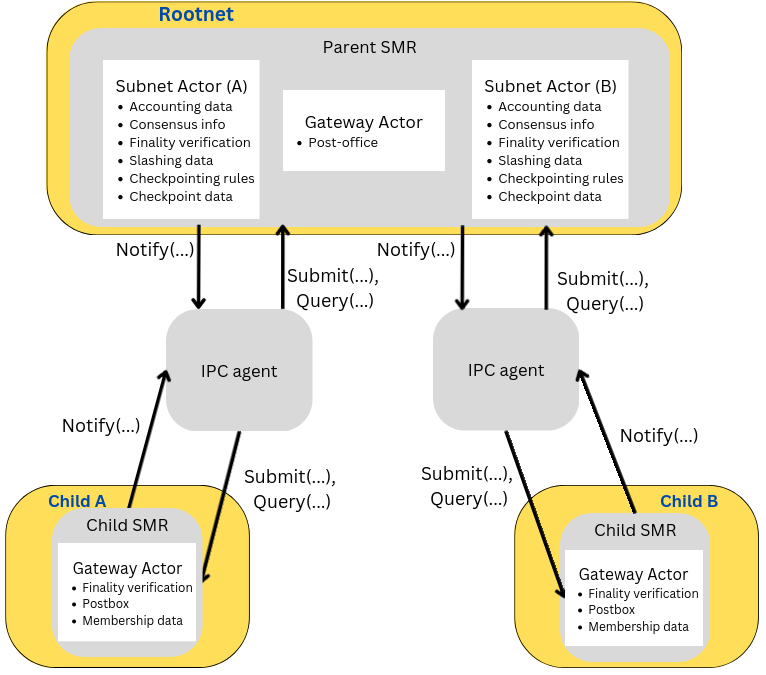
\includegraphics[width=0.75\textwidth]{compsintf-2subnets}
     \caption{The basic \ipc components and their interfaces in an example with one parent and 2 child subnets (A and B).}
     \label{fig:interfaces}
 \end{figure}


\paragraph{Incentives.}

In general, submitting transactions (and their subsequent execution by the subnet) is associated with a \emph{cost} (often referred to as ``gas").
We refer to the cost associated with a transaction as the \emph{transaction fee}, measured in coins.
A participant running an IPC agent is not necessarily interested in participating in such a costly protocol without incentives.
Moreover, the replicas of a subnet might need to cooperate with IPC agents during the construction of \pofsFull.
Even though certain deviations from the protocol can be detected and penalized (see \Cref{sec:slash}),
participants running subnet replicas might also need positive incentives to participate in the creation of a \pof.

The key to providing incentives for \ipc agents and replicas is that the \sa and the \gw can,
as actors, hold funds that their logic can distribute among other accounts or actors on their respective subnets.
Thus, the actors can be configured to reimburse an account associated with the \ipc agent submitting a transaction (potentially adding an extra reward), as well as to reward or penalize accounts.

The source of funding for the \gw and / or \sa is subnet-specific.
For example, a subnet’s implementation can require a certain part of each transaction fee to be sent to the subnet's \gw.
An \sa can be funded, for example, through transfers (withdrawals) of funds from the child subnet, or by charging fees for propagating cross-net transactions.

To incentivize the replicas of a subnet to collaborate with an IPC agent on the creation of \pofsFull, a similar mechanism can be deployed.
For example, a valid \pof would include metadata, where the replicas that participated in its creation could insert an address to receive a reward when the \pof is accepted.

\begin{example}
Our gaming platform from \Cref{sec:example-use-case} could use the following approach.
Each replica of the \subnetName{L2} subnet running the gaming platform is registered in the \gw of the subnet itself and has an associated account controlled by the participant operating the replica.
(Such a participant could be, for example, a local club of players who bought a server and are paying for internet connection.)
The \subnetName{L2} subnet is configured to pay a small fee to the \gw for each transaction executed by the subnet.
The \gw periodically (e.g., every 1000 blocks) re-distributes a part of the collected fees to the accounts associated with the replicas.

Each participant also controls an account in the rootnet (\subnetName{L1}) and operates an \ipc agent (e.g., running on the same machine as the replica)
to mediate the interactions between \subnetName{L1} and \subnetName{L2} (e.g., periodic checkpointing of \subnetName{L1}'s state to \subnetName{L2}).
The definition of \saOf{L2} requires a valid \pof to contain a withdrawal transaction transferring a certain amount of funds (e.g., from the \gw in \subnetName{L2})
to the \subnetName{L1} account associated with the \ipc agent submitting the \pof.
This way, the participant operating the \ipc agent has an incentive to submit the \pof.
To prevent too many or repeated submissions, the \saOf{L2} adjusts the reward based on the most recent \pof already submitted.

\end{example}

% \TODO{Add example of gaming system incentives: The replicas and \ipc agents running the \subnetName{L2} subnet might get a commission from transaction fees,
% while the single-game subnets might not need explicit incentivization at all, as they are mostly run by players, whose incentive is being able to play the game.}

 % - IPC Functionality
 %  - Minimum required per subnet
 %    - Withdrawal/Deposits Interfaces
 %    - Other Operations? (Propagate?)
 %  - Enhancements
 %    - Checkpointing interfaces
 %    - Propagate
 %    - Reporting/Slashing interfaces
 %    - Atomic execution/swap, IBC-like bridges
 %  - Future stuff (google docs?)
 %    - Withdrawal at ancestor (skip parent(s)) (with timeout) etc.
\section{IPC functionality}
\label{sec:functionality}
We list in this section the functionality that should be provided by the IPC components. We first list the minimal functionality required for every subnet (deposits and withdrawals), to then extend it with enhanced functionalities. We model components as processes that produce and consume events. Events consumed by the IPC agent are the result of either a notification from one of the SMRs or the response of a query made by the IPC agent. Events produced by the IPC agent result in the IPC agent submitting a transaction that will change the state of the SMR that consumes the event.

We note that our focus is on the core functionalities, disregarding optimizations for the moment. Batching is a prime example of this. It is expected that batching will be a key optimization whenever \verifyGfinal{\tx}{\prf} is used, as calling \verifyGfinal{\tx}{\prf} can be costly. Batching allows us to perform multiple operations for one \verifyGfinal{\tx}{\prf} call, reducing its overall cost.

\subsection{Minimal Functionality}
\label{sec:minFunc}
We show in this section the functionalities for deposits and withdrawals.

\subsubsection{Deposits}
\label{sec:deposit}

\arp{Consider need to pause/remedy subnet after deposit (e.g. collateral not enough with new supply). IPC agent should check in that case}\\

A deposit is a transfer of funds (of some amount \fil) from user $\user_P$'s wallet in the parent subnet to user $u_C$'s wallet in the child subnet.
We assume that $u_P$ is a participant running a parent replica, a child replica, and an \ipc agent.%
\footnote{If $u_P$ does not run these processes, $u_P$ contacts a trusted participant that does and that performs the deposit on $u_P$'s behalf.}
The deposit is performed by the user controlling the \ipc agent as follows:
\begin{enumerate}
    \item The local \ipc agent submits to the parent \smr replica the corresponding (properly signed) transaction
    $\tx=\textit{Deposit}\left( \src, \fil, \sa.\textit{accounts}.\dest \right)$ with $\src=\user_P$ and $\dest = \user_C$.
    \item The parent SMR system orders and executes the Deposit transaction (provided $u_P$ has enough funds) by transferring $amt$ from $u_P$'s parent account to the \sa (concretely, to $u_P$'s account representation within the \sa). This effectively locks the funds within the \sa \dapp, until the \sa \dapp transfers it back to $u_P$'s account during withdrawal (see \Cref{sec:withdraw}).
    \item When the parent's replicated state that includes the transaction becomes final (for some SMR-system-specific definition of finality), the local parent replica notifies the local \ipc agent, potentially attaching a proof of finality of $PoF(tx)$ to the notification.%
    \footnote{The exact content of $PoF(tx)$ depends on the implementations of the SMR systems. It might contain, for example, a quorum of replica signatures, a Merkle proof of inclusion, or even be empty.}
    \item The \ipc agent constructs a transaction $\tx' = \textit{Deposited}\left(\langle  \src, \fil, \sa.\textit{accounts}.\dest \rangle, \prf \right)$ and submits it to the child SMR system.
    \item Upon ordering $tx'$, the replicated logic of the child SMR system mints \fil new coins and adds them to $\user_C$'s account.
\end{enumerate}

We show in \Cref{fig:deposit} the events being produced and consumed by the deposit functionality and in Algorithm~\ref{alg:deposit} the pseudocode per component to implement the functionality.

\begin{figure}[h]
     \centering
     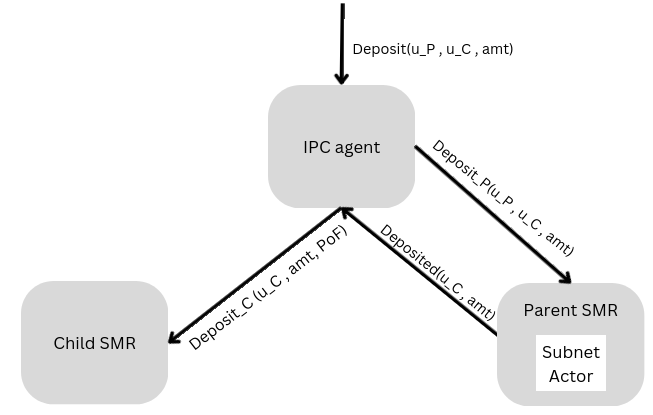
\includegraphics[width=\textwidth]{deposit}
     \caption{Events produced and consumed during a deposit.}
     \label{fig:deposit}
\end{figure}
 

\begin{algorithm}[H]
\footnotesize
\caption{Deposit operation}\label{alg:deposit}
  \DontPrintSemicolon
  \SetKwFunction{FMain}{Global}
  \SetKwProg{Pn}{Function}{:}{\KwRet}
  \SetKwInOut{Input}{input}
  \SetKwProg{Component}{$\blacktriangleright$ \bf}{:}{\KwRet}
  \SetKwFor{UponKW}{upon}{do}{fintq}
  \Input{\src account in parent, \dest account in child, amount~$\fil$}
   \Component{IPC agent}{
        submit $\tx=\textit{Deposit}\left( \src, \fil, \sa.\textit{accounts}.\dest \right)$ to parent \smr replica\;
  }
   %
   \Component{Parent \smr replica}{
   \UponKW{\tx}{
    move $\fil$ from \src to \sa.\textit{accounts}.\dest  \tcp*[r]{"lock" at parent}
    notify agent \texttt{ParentDeposited}(\tx)
   }
  }
  \Component{IPC agent}{
    \UponKW{notification of \texttt{ParentDeposited}(\tx) from parent \smr}{
        create \prf that \tx is final at parent \smr \tcp*[r]{see Sec.~? for details}
        submit \texttt{Deposited}$=\langle \tx, \prf \rangle$ to child \smr    
     }
  }
  \Component{Child \smr replica}{
    \UponKW{\texttt{Deposited}}{
        assert \prf for \tx\;
        increase \dest account by \fil
     }
  }
\end{algorithm}
One thing that differs a downward transaction (e.g., deposit) from an upward transaction (e.g., checkpoint) is that any participant that operates the child \smr replica also has visibility into the state of the parent \smr (albeit stale) through its local parent \smr replica. This enables the \textbf{local validity check} method to assert the finality at the parent (which may or may not be preferred over others).%
\footnote{\textbf{local validity check} (simpler, efficient, \textit{weaker guarantees}): $\prf$ contains a pointer to the block containing \tx  at the parent, together with the height~$h$ of that block.
 To assert that \tx is final, the child queries the parent about $TX$, if it exists -- return valid, else -- return invalid. If invalid but the parent is still below height~$h$, then query again when parent reaches height~$h$.
This is a test inside the child \smr process. Therefore, if we want this method (and I believe we do), we should widen the interface so that a child \smr can ask the agent to get data from the parent. However, this optimization comes at the expense of the encapsulation of components, that is, it entails tinkering with the child \smr code.}
            
\subsubsection{Withdrawals}
\label{sec:withdraw}

A withdrawal is a transfer of funds from user $u_C$'s wallet in the child subnet to some user $u_P$'s wallet in the parent subnet. We assume that $u_C$ is a participant running a parent replica, a child replica and an \ipc agent. The withdraw is performed as follows:
\begin{enumerate}
  \item $u_C$ triggers the $Withdraw(u_C, u_P, amt)$ event at the local \ipc agent.
    \item The local \ipc agent submits the corresponding (properly signed) transaction $tx = Withdraw_C(u_C, u_P, amt)$ to the child SMR system.
    \item The child SMR system orders and executes the Withdraw transaction, burning $amt$ funds in $u_C$'s account (provided $u_C$ has enough funds).
    \item When the child's replicated state that includes the transaction becomes final (for some SMR-system-specific definition of finality that has been defined in the SA), the local child replica notifies the local \ipc agent, potentially attaching a proof \prf that this state is final.%
    \item The \ipc agent constructs a transaction $tx' = Burned(u_P, amt, \prf)$ and submits it to the parent SMR system.
    \item Upon ordering $tx'$, the replicated logic of the parent SMR system updates the state of the SA transferring the funds from \sa (concretely, to $u_P$'s account representation within the \sa) to $u_P$'s account.
\end{enumerate}

 \begin{figure}[h]
     \centering
     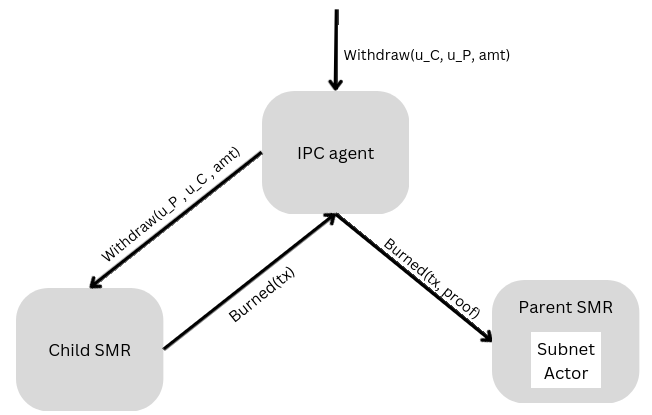
\includegraphics[width=\textwidth]{withdrawal}
     \caption{Events produced and consumed during a withdrawal.}
     \label{fig:withdrawal}
 \end{figure}
\begin{algorithm}[H]
\footnotesize
\caption{Withdraw operation}\label{alg:down}
  \DontPrintSemicolon
  \SetKwFunction{FMain}{Global}
  \SetKwProg{Pn}{Function}{:}{\KwRet}
  \SetKwInOut{Input}{input}
  \SetKwProg{Component}{$\blacktriangleright$ \bf}{:}{\KwRet}
  \SetKwFor{UponKW}{upon}{do}{fintq}
  % \Input{user~$\user$, amount~$\fil$, transaction \txnf}
   \Input{\src account in child, \dest account in parent, $\fil$ amount of coins}
   \Component{IPC agent}{
        submit $\tx=\textit{Withdraw}(\src, \fil, \dest)$ to child \smr\;
  }
   %
   \Component{Child \smr replica}{
   \UponKW{$\tx = \textit{Withdraw}(\src, \fil, \dest)$}{
    deduct $\fil$ from \src account at child \tcp{``burns" \fil in child}
    notify agent \texttt{Burned}(\tx)
   }
  }
  \Component{IPC agent}{
    \UponKW{notification of \texttt{Burned}(\tx) from child \smr replica}{
    
        create \prf that \tx is final at child \smr \tcp*[r]{see Sec.~? for details}
        submit $\tx'=\texttt{Burned}\left(\tx, \prf \right)$  to parent \smr replica
     }
  }
  \Component{parent \smr replica}{
    \UponKW{$\tx'=\texttt{Burned}\left(\tx, \prf \right)$}{
        assert \sa.\verifyGfinal{\prf}{\tx}\;
        move \fil coins from \sa.accounts[\src] to \dest
     }
  }
   
%    \Component{Child SMR}{
%    [\tx submitted by user, proposed, written]\\
%    \UponKW{\txnf written in Child SMR}{
%     decrease user fund's by $\fil$\\
%     Send \texttt{ChildWithdrawn(\tx, [$proof$])} to IPC agent \tcp*[r]{notify IPC agent}
%    }
%   }
%   \Component{IPC agent}{
%     \UponKW{\texttt{ChildWithdrawn(\tx, [$proof$])} notified by Child SMR}{
%     \If{$proof=$ \textbf{nil}}{
%          $proof \gets $\textit{generateProofOfGlobalFinality(\tx,...)} \tcp*[r]{Necessary steps for \tx to be ready to be submitted to Parent SMR}
%      }
%      \texttt{ChildWithdrawn(\tx, $proof$)} to parent SMR \tcp*[r]{Submit to parent}
%      }
%     \UponKW{\arp{State updated after Withdrawal}}{ \tcp*[r]{Notified when parents update state}
%       \arp{Check child subnet rules are still satisfied, remedy/close otherwise?}
%     }
%   }
%   \Component{Parent SMR}{
%   \UponKW{\texttt{ChildWithdrawn(\tx, $proof$)} submitted by IPC agent}{
%       \If{\sa.\verifyGfinal{\tx}{\prf}}{
%            [tx submitted by IPC agent, proposed, written]\\
%            \UponKW{\txnf written in Parent SMR}{
%                 reduce $\fil$ amount for user $\user$ in SA\\
%                 Parent SMR notifies IPC agent
%             }
%       }
%   }
% }
\end{algorithm}
\subsection{Enhanced Functionality}
\label{enhancedFunc}
\arp{From here below we need to add the gateway actor and refine the functionality, leave out till round of feedback for GW}
We show here a list of desirable functionalities that build upon the basic withdrawals and deposits.
\subsubsection{Checkpointing} A checkpoint contains a representation of the updated state of the child SMR system to be included in the parent SMR system. A checkpoint can be triggered by predefined events (i.e. periodically after a number of state updates, triggered by a specific user or set of users, etc.). As such, the checkpoint functionality may or may not be triggered by a user request on the child SMR. A checkpoint is performed as follows: 
\begin{enumerate}
\item If the predefined checkpoint trigger is met, then the IPC agent queries the child SMR replica for the updated state to be represented in this checkpoint.
\item The IPC agent creates a proof \prf that this updated state of the child SMR system is final, possibly compressing its representation of the state.
\item The IPC agent submits a transaction $\tx'=\texttt{Checkpoint}\left(\textit{state}, \prf \right)$ to the parent SMR replica
 \item Upon ordering $tx'$, the replicated logic of the parent SMR system updates the state of the SA according to the checkpoint state, if necessary.
\end{enumerate}

\begin{figure}[h]
     \centering
     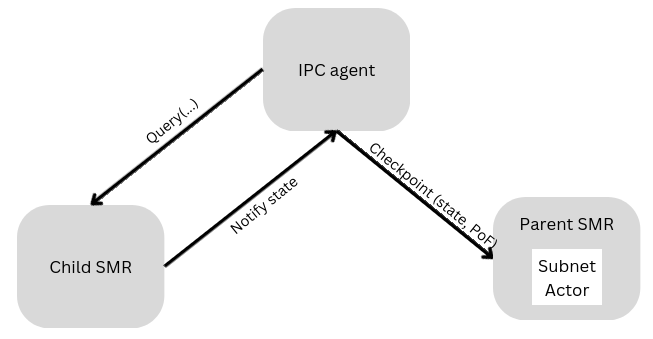
\includegraphics[width=\textwidth]{checkpoint.png}
     \caption{Events produced and consumed by the checkpointing functionality.}
     \label{fig:chkp}
 \end{figure}
\begin{algorithm}[H]
\footnotesize
\caption{Checkpoint operation}\label{alg:down}
  \DontPrintSemicolon
  \SetKwFunction{FMain}{Global}
  \SetKwProg{Pn}{Function}{:}{\KwRet}
  \SetKwInOut{Input}{input}
  \SetKwProg{Component}{$\blacktriangleright$ \bf}{:}{\KwRet}
  \SetKwFor{UponKW}{upon}{do}{fintq}
   \Component{IPC agent}{
        \If{trigger for checkpoint}{
            \textit{state} $\gets$ query the child \smr replica for the state\;
            create \prf that \textit{state} is final at child \tcp*[r]{Possibly compress \textit{state}}
        }
        submit $\tx'=\texttt{Checkpoint}\left(\textit{state}, \prf \right)$  to parent \smr replica
  }
  \Component{parent \smr replica}{
    \UponKW{$\tx'=\texttt{Checkpoint}\left(\textit{state}, \prf \right)$}{
        assert \sa.\verifyGfinal{\prf}{\textit{state}}\;
        $\sa.\textit{latestCheckpoint} \gets \textit{state}$
     }
  }
  
  % \Input{[User's checkpoint request]}
  % \Component{Child SMR}{
  %    \UponKW{State updated [ \textbar User's checkpoint request]}{ 
  %       [Write checkpoint request if any]\\
  %      Send \texttt{StateUpdated($st$)} to IPC agent \tcp*[r]{Notify IPC agent}
  %    }
  % }
  % \Component{IPC agent}{
  %   \UponKW{\texttt{StateUpdated($st$)} notified by child SMR}{
  %       \If{\texttt{SatisfiesCheckpointCondition($st$)}}{
  %          Create checkpoint \chkp\\
  %           $proof \gets $\textit{generateProofOfGlobalFinality($st$,...)} \tcp*[r]{Necessary steps for \tx to be ready to be submitted to Parent SMR}
  %           Submit \texttt{SubmitCheckpoint(\chkp)} to parent SMR
  %           }
  %       }
  % }
  % \Component{Parent SMR}{
  %     \UponKW{\texttt{SubmitCheckpoint(\chkp)} submitted by IPC agent}{
  %        [\chkp proposed, written]\\
  %        Refund fee to submitter \tcp*[r]{refund at parent for simplicity}
  %     }
  % }
\end{algorithm}

\subsubsection{Slashing} 
\guy{This section is immature for review (even a preliminary one)}\\
We show here the events produced and consumed by the slashing functionality. Given specific misbehavior from participants that is identified as Proofs of Fraud (PoFs), e.g.
gathering signed equivocating messages, the child SMR reports the PoFs to the IPC agent, which immediately forwards a slash a request to the parent SMR. \arp{Extend with need to verify if child SMR can continue, needs to remedy its depleted collateral or should be killed with latest checkpoint/state update}.
\begin{figure}[h]
     \centering
     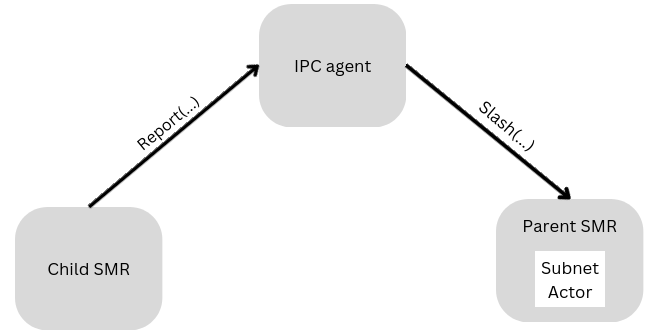
\includegraphics[width=\textwidth]{slash}
     \caption{Events produced and consumed by the slashing functionality.}
     \label{fig:report}
 \end{figure}\\

\begin{algorithm}[H]
\footnotesize
\caption{Slash Functionality}\label{alg:down}
  \DontPrintSemicolon
  \SetKwFunction{FMain}{Global}
  \SetKwProg{Pn}{Function}{:}{\KwRet}
  \SetKwInOut{Input}{input}
  \SetKwProg{Component}{$\blacktriangleright$ \bf}{:}{\KwRet}
  \SetKwFor{UponKW}{upon}{do}{fintq}
  \Input{-}
  \Component{Child SMR}{
     \UponKW{Proofs of fraud \pofs generated}{
       Notify \report to IPC agent
     }
  }
  \Component{IPC agent}{
    \UponKW{\report notified by child SMR}{
        Submit \slashop to parent SMR
    }
    \UponKW{\arp{State updated after slashing}}{
      \arp{Check child SMR rules are still satisfied, remedy/close otherwise?}
    }
  }
  \Component{Parent SMR}{
        \UponKW{\slashop submitted by IPC agent}{
         Update SA state slashing/excluding participants
         Notify SA update to IPC agent
        }
  }
\end{algorithm}


\subsubsection{\postoffice}
The \postoffice functionality is an inter-subnet transaction service. The main motivation for this functionality comes from a ``potential clients" request: enable a \dapp in one subnet to interact with a \dapp in a different subnet.\\
\guy{Edge case: a leaf subnet does not have a \sa and, therefore, no \postoffice. We can consider removing the \postoffice functionality from the \sa and to deploy it as an independent \dapp that will appear only once per subnet. In this case, it needs permissions to call \sa.\verifyGfinal{\tx}{\prf} function.}

\begin{algorithm}[H]
\footnotesize
\caption{\postoffice Functionality}\label{alg:po}
  \DontPrintSemicolon
  \SetKwFunction{FPropagate}{propagate}
  \SetKwProg{Pn}{Function}{:}{\KwRet}
  \SetKwInOut{Input}{input}
  \SetKwProg{Component}{$\blacktriangleright$ \bf}{:}{\KwRet}
  \SetKwProg{Empty}{\bf}{:}{\KwRet}
  \SetKwFor{UponKW}{upon}{do}{fintq}
  \Input{$\tx = \langle \data, \src, \dest, \prf \rangle$}
  \Component{\sa.\postoffice}{
     \UponKW{\postoffice.\propagate(\tx) }{
       \Case{\dest in current subnet}{
            \postoffice.\propagate\textit{HERE}(\tx)
       }
       \Case{\dest requires going up the tree}{
            \postoffice.\propagate\textit{UP}(\tx)
       }
       \Case{\dest requires going down the tree}{
            \postoffice.\propagate\textit{DOWN}(\tx)
       }
     }
     \UponKW{\postoffice.\propagate\textit{UP}(\tx) }{
       \If{\src not from this subnet}{
            assert(\sa.\verifyGfinal{\tx}{\prf})\;
       }
       \src.\textit{append(\sa's subnet id)}\;
       emit event \postoffice.UP$\langle \data, \src, \dest \rangle$
     }
     \tcp{\propagate\textit{DOWN}(\tx) is analogous to \propagate\textit{UP}(\tx)}
     \tcp{\propagate\textit{HERE}(\tx) is trivial}
  }
  \Component{parent \smr process}{
     \UponKW{event \postoffice.UP$\langle \data, \src, \dest \rangle$}{
        $\tx \gets \langle \data, \src, \dest \rangle$\;
        notify agent on \postoffice.UP(\tx)
     }
  }
  \Component{IPC agent}{
    \UponKW{notification of \propagate\textit{UP}(\tx) from child \smr}{
        create \prf that \textit{UP}(\tx) is final at child \smr\;
        $\tx_\textit{new}\gets\langle \textit{UP}(\tx), \prf \rangle$\;
        submit \sa.\postoffice.\propagate($\tx_\textit{new}$) to parent \smr
    }   
}
\end{algorithm}
\subsubsection{Atomic Execution}
TODO Discuss in Lanzarote?


\subsection{Future}
\label{sec:future}
 % - Components and their Interfaces
 %   - Parent subnet node
 %   - Child subnet node
 %   - IPC module
 %   - Subnet actor
 \section{Components and their Interfaces}
 \label{sec:components}

In \ipc, whole subnets need to interact.
I.e., the replicated state of one subnet must react to (changes in) the replicated state of another subnet.
As the replicated state of every subnet is distributed among its replicas and evolves independently of other subnets,
we must establish a mechanism for interactions between the states of subnets.
In particular, we must explicitly link the two replicated states of two subnets.
More precisely, for any interaction between two subnets ($A$ and $B$), define block heights $h_A$ and $h_B$,
such that $A$'s replicated state at height $h_A$ considers $B$'s replicated state to have evolved exactly until $h_B$.

To this end, we define a \emph{\pofFull (\pof)} to be data that proves that an SMR system definitively reached a certain replicated state.
Regardless of the SMR system's ordering protocol's approach to finality (e.g., immediate finality for classic BFT protocols, or probabilistic finality in PoW-based systems),
a \pof convinces the the proof's verifier that the replicated state it refers to will not be rolled back.
We denote by \emph{\pof(tx)} the proof that an SMR system reached a state in which transaction \emph{tx} already has been applied.
For example, for a BFT-based SMR system, a quorum of signatures produced by its replicas can constitute a \pof.



We separate the software needed to run \ipc into three processes and two \dapps:

\matej{\todo{Express those components and their interfaces also in pseudocode.}}
\begin{enumerate}
    \item \textbf{\ipc agent:} The software that is in charge of the interactions between the two blockchains. This includes, for example, observers for the parent and child subnets. (Note that it is a process and not a smart contract). The \ipc agent is a piece of software that mediates the interactions between the child and parent \smr software modules.    
    \item \textbf{Parent \smr replica:} The software that runs the parent blockchain. Note that this module also entails the interaction with the \ipc smart contract~\sa, which is maintained at the parent subnet. Any update that the parent process performs on \sa is notified to the \ipc agent.
    \item \textbf{Child \smr replica:} The software that runs the child blockchain. Note that some of the rules the child blockchain must satisfy are listed in~\sa. Any output operation (withdraw, checkpoint) is notified to the parent process through the \ipc agent. 
%    \item \textbf{IPC smart contract / subnet actor (\sa):} The smart contract implementation that is running on the parent blockchain. It is invoked only through transactions that are included in the parent blockchain.
    \item \textbf{IPC subnet actor (\sa):} The smart contract implementation that is running on the parent blockchain. It is invoked only through transactions that are included in the parent blockchain.
    \item \textbf{IPC coordinator/gateway actor (\gw):} a smart contract that exists in every non-leaf subnet in the \ipc hierarchy and contains methods facilitating inter-subnet operations.	
\end{enumerate}


We now define minimal interfaces between the different modules that enable the correct operation of an \ipcFull system.
A guiding principle in the interface design is to minimize changes to the \smr codebase; therefore, most extra logic of the \ipc will be added into the \ipc agent and the smart contracts \sa~and~\gw. Doing so should facilitate the deployment of \ipc with new \smr protocols by not requiring a developer familiar with \ipc to be an expert on \smr: some understanding is still needed to optimize the agent's implementation, but the \smr code would remain portable.

We require four interfaces: (i) \ipc agent --- parent \smr, (ii) \ipc agent --- child \smr, (iii) parent \smr --- \sa, and (iv) any \smr --- \gw. Both (i) and (ii) can comprise of only:
\begin{enumerate}
    \item Agent submits a transaction~\tx to the \smr process.%
    \footnote{As part of the notification defined below, it could be that after submitting \tx, until the \smr process returns \textit{complete} (perhaps with a finality parameter) or \textit{declined}, \tx is considered \textit{pending}.}
    \item Agent queries the state of the \smr process. The \smr process returns its current state (possibly limited to only a requested part of the state).
    \item \smr process notifies the agent on events of interest (e.g., changes to the state of~\sa).
\end{enumerate}

The interface between an \smr and~\sa or~\gw is based on the execution engine of that \smr and the functionality desired by~\sa. The specifics of the execution engine's system calls depend on implementation. Whenever such a call is not clear from context we provide a description of what it entails. \\


\T{The state of \sa includes representations of:}
% accounting
% Consensus functionality
% functionalities: proofOfFinality
\begin{itemize}
    \item Accounting data. This can vary from a single account representing all the parent's coins in the child to an account balance for each user in the child subnet (custodial vs non-custodial accounting). We continue with the non-custodial approach as the other can be viewed as a specific limitation of it.
    %
    \item Governance account (denoted \gov). This account facilitates the economic design of a subnet. It can be used for governing operations of the subnet. For example, collecting fees and making payments (to validators, for checkpoint reimbursement etc.) 
    %
    \item Consensus information. The data (or a pointer to it) that is needed to run the ordering of the subnet.
    \begin{itemize}
        \item Consensus protocol.
        \item Subnet configuration such as the validator set, voting rights, collateral deposits, etc.
        \item Payments methods for participation. E.g., transaction fee mechanism, block rewards.
    \end{itemize}
    %
    \item Finality verification. A method to Verify that a state/\tx is final%
    \footnote{Finality is an elusive concept that we do not take upon ourselves to define here. For simplicity, we assume finality in a Boolean manner, either \tx is final or it is not. This could easily be generalized to parameterized finality of the sort ``the probability of \tx persisting is at least~$x$."}
    in the child subnet. For this, we will use the function \sa.\verifyGfinal{\tx}{\prf} which excepts as arguments a transaction (or state) and a \prf, and outputs True if \tx is considered globally final in the child subnet and False otherwise. This function must only depend on its inputs and the internal state of~\sa. For example, \prf is a threshold signature that can be verified against the set of validators in~\sa.
  \item Parent's finality verification. A method to verify that a state/\tx is final in the parent subnet. For this, we will use the function \gw.\verifyPfinal{\tx}{\prf} which excepts as arguments a transaction (or state) and a \prf, and outputs True if \tx is considered globally final in the parent subnet and False otherwise. This function must only depend on its inputs (and perhaps some internal state of~\gw). \arp{subnet specific, not necessarily the same method for all child subnets. Lives at the SA (needed for deposits but deposits should not depend on \gw)}
\end{itemize}
%
The above suffices for an \ipcFull system with a minimal inter-subnet functionality of users' asset-transfer, and a general \smr per subnet. We continue with the additional state required for enhanced functionalities.
%
\begin{itemize}
    \item Slashing functionality.
    \begin{itemize}
        \item List of slashable misbehaviors and a proving methodology. That is, for each slashable misbehavior there is a definition of what constitutes a valid proof of misbehavior (\pom).
        \item Incentives design, i.e., specified penalties for misbehavior and rewards for reporting.
    \end{itemize}
    %
    \item Checkpointing rules.
    \begin{itemize}
        \item When checkpoints are valid. E.g., every~$\Delta$ subnet-blocks from the previous checkpoint, or the checkpoint's $L_2$ distance from the previous is larger than~$L$.
        \item Fee payments for checkpoints.
    \end{itemize}
    %
%    \item Inter-subnet transactions service (denoted \postoffice). 
%    \sa contains functionality that can be used to transfer data from one subnet to another. In particular, consider the following case involving a smart contract.%
%    \footnote{When inter-subnet data transfer happens between users (Externally Owned Accounts --- \eoa --- in Ethereum's jargon), they can actively participate in the propagation via the \ipc agent that communicates with both the parent and child subnets. Smart contracts, on the other hand, do not have that power and, therefore, cannot communicate inter-subnets as efficiently as users (\eoa).}
%    Smart contract $\textit{SmCt}$ emits an event~$e$ that contains $\textit{data}$ which is desired to reach the destination~\textit{dest} in a different subnet.
%    The \postoffice specifies the methods and the state locations that are used by this service.
\end{itemize}
Recall that \sa lives at the parent \smr. However, some of the objects that are represented in \sa are modified in the child subnet (e.g., accounting data). Therefore, such objects are likely to have a representation in the child \smr as well.
Moreover, the representation in the child \smr may differ from those in~\sa. This is due to \sa being less frequently updated (it is part of the parent \smr state). The representations are periodically synchronized, e.g., at a checkpoint event. \Cref{fig:interfaces} illustrates the components and their interfaces.\\


% We remark that all of the above are likely to have representations in the child \smr as well. Moreover, the representation in the child \smr may differ from those in~\sa. This is due to \sa being less frequently updated (it is part of the parent \smr state). The representations are periodically synchronized, e.g., at a checkpoint event. \Cref{fig:interfaces} illustrates the components and their interfaces.
\begin{figure}[h]
     \centering
     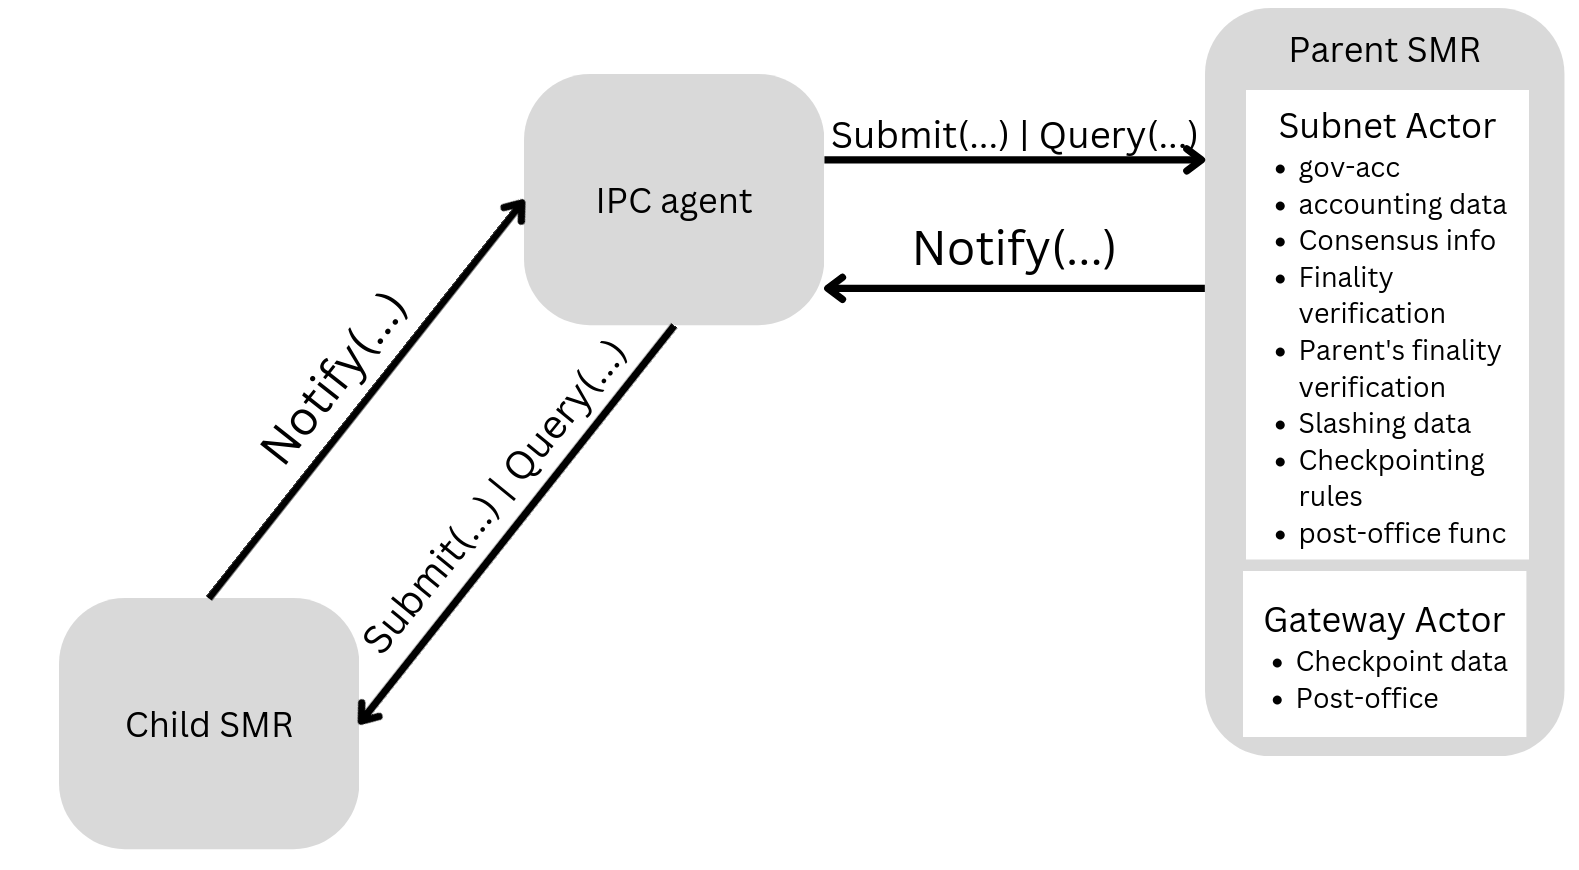
\includegraphics[width=0.75\textwidth]{compsintfs}
     \caption{The basic components and their interfaces.}
     \label{fig:interfaces}
 \end{figure}


\T{The state of \gw includes:}
\begin{itemize}
    \item Checkpoint data. The parent stores at the \gw each of the checkpoints from each direct child of it.
    \item Inter-subnet transactions service (denoted \postoffice). 
    \gw contains a registry of subnets and a functionality that can be used to transfer data from one subnet to another. 
    The \postoffice specifies the methods and the state locations that are used for these services.
    In particular, consider the following case involving a smart contract.%
    \footnote{When inter-subnet data transfer happens between users (Externally Owned Accounts --- \eoa --- in Ethereum's jargon), they can actively participate in the propagation via the \ipc agent that communicates with both the parent and child subnets. Smart contracts, on the other hand, do not have that power and, therefore, cannot communicate inter-subnets as efficiently as users (\eoa).}
    Smart contract $\textit{SmCt}$ emits an event~$e$ that contains $\textit{data}$ which is desired to reach the destination~\textit{dest} in a different subnet.
\end{itemize}
 
 
 
\section{Related Work}
\label{sec:related-work}

    We categorize related work in the following subcategories of approaches to scale blockchains: novel consensus protocols, rollups, channel networks, and subnet networks (like IPC). Note however that   these categories are not inherently competing, but rather potentially orthogonal solutions that, carefully combined, could scale even beyond what one of them, in isolation, is capable of.  
    \subsection{Consensus protocols} Recent developments in asynchronous consensus protocols have significantly increased throughput by decoupling data dissemination from metadata ordering~\cite{keidar2021DAG, spiegelman2022Bullshark, Narwahl, Lu2020Dumbo, Lu2022Bolt, Lu2022Dumbo, aptoslabs, hedera, sui,ISS}. These advances are inherently restricted by the need to replicate all state updates across all members of the consensus protocol. Furthermore, their improvements are orthogonal to the horizontal scaling proposed by IPC, in that each subnet can benefit from these advances at their consensus level. 
    
    \subsection{ZK and optimistic rollups} Rollups scale blockchains by having third parties (sequencers) locally order and execute batches of transactions and submitting only the result of the batch in the blockchain. Optimistic rollups~\cite{kalodner2018arbitrum, rollmint} rely on the result of a sequencer allowing for a predefined dispute period. If disputed, the sequencer is not punished only if it proves within a limited amount of time, via executing the batch in the blockchain, that the result of its batch matches its submitted result. ZK rollups~\cite{nazirkhanova2021information, appliedzkp, polygon-zkevm, starkware, sin7y, matterlabs, appliedzkp, espressosys} cryptographically generate a succinct proof of the correctness of the result for fast verification. Unfortunately, most ZK rollups proposed to date rely on centralized sequencers, with some novel works working on decentralizing sequencers~\cite{espressosys}. In addition, rollups that  post transaction input data on L1 inherit throughput scalability limitations of an L1. Some alternative approaches such as Validium \cite{Validium}, combine ZK rollups with input data storage off-L1, for better scalability. 

    Compared to rollups, \ipc to a certain extent resembles a combination of Validium and optimistic rollups in a sense that \ipc subnets leverage parent subnets for increased security, while storing transaction data off parent subnet, i.e., in a child subnet itself, replicated with a BFT protocol. \ipc currently does not use ZK technology for transaction execution in subnets; however, such support is not precluded in future. In particular, our group aims at exploring integration of Lurk ZK execution framework \cite{Lurkpaper} in \ipc subnets. 
    
    \subsection{Sharding} Sharding~\cite{zamani2018rapidchain, Leftheris2018Omniledger, Luu2016Shards, Yu2020Survey, avarikioti2021divide, androulaki2018Channels, wang2019monoxide, albassam2017chainspace, hong2021pyramid} approaches periodically partition blockchain state across different groups of replicas. While sharding has shown promise in increasing scalability, it also introduces new challenges such as ensuring cross-shard communication and preventing data fragmentation. Unlike subnets, shards do not conceptually differ from each other, leading to a potential increase of cross-shards communication compared to subnets, where users and services partition the state on demand.
    
    \subsection{State and payment channels} State channels~\cite{dziembowski2018general} scale blockchains by having participants lock their state in the blockchain (on-chain) among them in order to update locally the state (off-chain) with which to release the funds back on-chain. Payment channels~\cite{poon2016bitcoin, decker2015fast, burchert2018scalable} are the analogous solutions for channels where the state are coins. Channels can form network graphs in which nodes can relay payments (or general state) in exchange of a fee~\cite{lnd2018, BOLT, network2023raiden, clightning2023, eclair}. Though many works, particularly in state channels, are addressing significant problems specific to channels, IPC subnets are a generalization of channels. This is because channels require all parties to sign in order to update the channel's state off-chain, whereas subnets (like the ones we show in this document) allow for a variable quorum size, or even different types of proofs of finality.

    \subsection{Subnet and sidechain networks}
    There are a number of previous and concurrent works that are conceptually similar to IPC subnets. 
    
    \paragraph{Single-layer networks.} Polkadot's relay-chain connects Polkadot's parachains~\cite{polkadotparachains} with native cross-net transactions, in a topology that also resembles a single scaling layer of direct child subnets of a rootnet. They also offer specialized bridges to other blockchains, like that of Bitcoin or Ethereum. Polkadot's parachains rely on anchoring their compressed state to the parent for total ordering and cross-net interactions, which limits the capabilities of horizontal scaling: parachains need to constantly lease an auctioned slot on the relay-chain for a specific period, a problem that is exacerbated in a single layer of child subnets checkpointing to the same parent, compared to IPC's tree topology. Polygon~\cite{polygonpos, polygonsupernets} scales the Ethereum blockchain by using a network of subnets (sidechains in the Polygon terminology) connected to the Ethereum mainnet, with a developing framework for services to create their own subnet. Yet, Polygon PoS offers one subnet, and Polygon does not offer a native cross-net communication protocol. Avalanche offers a similar solution for its rootnet with Avalanche subnets~\cite{avaxsubnets}, a network of subnets that are connected to their rootnet for further scaling and customized applications. 
    % \jorge{As pointed out by Marko, this is no longer true: https://medium.com/avalancheavax/avalanche-warp-messaging-awm-launches-with-the-first-native-subnet-to-subnet-message-on-avalanche-c0ceec32144a . There are still differences, e.g. their mechanism seems to lack the same properties and also the lack of hierarchy}\arp{Updated accordingly}
    Internet Computer Protocol's (ICP) subnets~\cite{icp} are independent blockchains with the ICP rootnet as the common parent, and whose committees are subcommittees of the rootnet's validator set. ICP subnets are tightly integrated with its rootnet and dedicated to execute smart contracts seamlessly. Unfortunately, none of these works consider a structure beyond a single layer of direct child with their respective rootnet as the only parent. 

    \paragraph{Topology-agnostic networks.} The concept of sidechains~\cite{back2014enabling, gazi2019proof} precedes that of subnets. In particular, \ipc parent-child interaction design and \ipc trust model, draws a lot of inspiration from PoS sidechain formalization \cite{gazi2019proof}. A sidechain targets crosschain payments not necessarily in the parent-child hierarchy. Cosmos zones~\cite{cosmosdocs} are independent blockchains that interact in a general graph not necessarily in the topology of a tree, with a reference implementation that spawns new zones running Tendermint as the consensus protocol. Cosmos relies on the single finality of Tendermint for inter-blockchain communication (IBC). Cosmos zones can alternatively use the Cosmos hub, a zone that specializes in facilitating cross-net interactions, similarly to the Polkadot relay-chain. The flexibility for any topology between subnets comes with the need to have further requirements for IBC, like having nodes of a blockchain run light clients of each other blockchain they want to interact with.

    \paragraph{UTXO-based subnets.} Plasma chains~\cite{poon2017plasma} horizontally scale payments via multiple subnets (childchains) organized in a tree-like structure. It is, one of the first works to consider subnet-like interactions between blockchains. Given the topology, many of the challenges that IPC subnets face are present in Plasma chains. However, Plasma chains are tree-based subnets focused on payments. In this sense, IPC subnets generalize the problem that Plasma chains are trying to solve, allowing state to be transacted in subnets, and not just payments. Also, Plasma chains rely on synchrony for withdrawals offering a dispute resolution period, similarly to channels and optimistic rollups, posing an irreconcilable trade-off between finality latency and security~\cite{platypus2019ranchalpedrosa}, with Platypus~\cite{platypus2019ranchalpedrosa} approaching the \pof shown for IPC subnets running Trantor as the first fix to this trade-off. IPC subnets also generalize withdrawal mechanisms by allowing subnets to define what constitutes a \pof, a slashing rule and a fraud proof. 
    
% \noindent\textbf{Plasma chains:}
% \begin{itemize}
%     \item A similar tree topology of subnets where a child subnet is rooted at the parent.
%     \item Additional security by committing to the parent cryptographic proofs for the validity of state transitions of the child.
%     \begin{itemize}
%         \item For a payment subnet in the UTXO model, this can be done with Merkleized proofs. It is relatively efficient, and we should consider (in the future) developing an off-the-shelf subnet that does it.
%         \item For general purpose subnets a more complex proving system is required (e.g., ZK proofs).
%     \end{itemize}
%     \item The added complexity of the additional security (that roughly equals to the parent security) manifests itself at withdrawals. Withdrawing (moving funds from the child to the parent) requires substantial time delay to allow challenges to the validity of the withdrawal. The need to challenge malicious withdrawals also implies additional effort from the participants which need to be vigilant to ensure the system’s safety.
%     \item Plasma relies upon users detecting Byzantine block withholding behavior, the users are responsible for exiting the Plasma blockchain quickly in case they detect such a behavior. 
%     \item Plasma does not conflict with our design. We could (and probably should in the future) add a reference implementation for deploy a plasma subnet.
% \end{itemize}
% \paragraph{Avalanche subnets.}
% \begin{itemize}
%     \item Single layer (not recursive) – all part of the primary network.
%     \item Flexible consensus (like ours).
% 	\item Also flexible execution engine possible.
% 	\item Do not use the parent for increased security (staking in the subnet and coins are minted internally with no need to deposit at the parent.)
% 	\item Inter subnet communication via (3rd party) bridges.
% \end{itemize}

% \paragraph{Polkadot subnets:}
% \begin{itemize}
% 	\item A sharded blockchain in the classic sense. Basically, it’s a single blockchain containing the “headers” of each block of each parachain. (Parachain==subnet.)
% 	\item Everything goes through the main chain (“relay chain”). It uses erasure codes and Merkle roots for efficiency.
% 	\item It is a single layer
% 	\item All security relies on the main chain with random assignment of validators to parachains.
% 	\item Built-in inter subnet communication via the relay chain (after all, it is the source of truth for all and each block).
% \end{itemize}

% \paragraph{Cosmos subnets:}
% \begin{itemize}
% 	\item Most similar to us
% 	\item The purpose of Tendermint is roughly like the purpose of Trantor in our eco-system. That is, a plugin parametrized consensus engine.
% 	\item The cosmos subnets topology is more flexible than our tree structure. (A general graph.)
%     \item The graph edges in Cosmos are based on bridges between any two subnets (hence no hierarchy and more trust requirements). These bridges can be an additional (future) application on top of our system, so there is no conflict.
% 	\item They also have in their eco-system a special “subnet” called the hub. The hub is an implementation of a subnet that specializes in facilitating inter-blockchain communication among multiple other subnets (in a similar fashion to the Polkadot relay chain).
% 	\item I could not find clear incentives arguments for the cross subnet communication through a hub (multi-hop).
% \end{itemize}


% \noindent\textbf{Polygon PoS (Matic):}
% \begin{itemize}
%     \item Ethereum compatible, with general EVM transactions (not only asset transfer).
%     \item It claims to be a Plasma side chain.
%     \item I did not understand how this is done while maintaining the Plasma guarantees (i.e., verification of every child transaction at the parent) since they did not add ZK mechanisms inside.
% \end{itemize}



% \noindent\textbf{ICP subnets:}
% \begin{itemize}
    % \item single layer, no parent -> no checkpointing to parent (less security).
% \end{itemize}
 % - Implementations/templates
 %  - Different types and trade-offs of checkpoint triggers 
 %    - Periodically: time, #blocks, #withdrawn, etc.
 %    - At request: (this one is not governance funded)
 %    - Combinations of these 
 %    - Slashing functions
 %    - Atomic execution types?
 \section{IPC's reference implementation}
 \label{sec:ref-impl}
 
% \jorge{I like the idea of the section but it currently reads a little weird, particularly beyond 8.1. There is this list of components/topics and a number of entries under them, but no narrative and, for many of the entries, it's unclear whether the implementation details actually add useful details, vs. just repeating the design or listing implementation "facts" without explaining their relevance. I don't know if the solution is less content of more content, but I might start with making it less "entry"-based and more narrative, focusing on things that are either very relevant/important os potentially unexpected and hence deserving of an explanation. I think e.g. 8.4 (incentives) is written in a more useful style.}

 The reference implementation of IPC differs slightly from the description of the functionality and implementation shown in previous sections, partly due to the rapidly changing development of the system, and partly due to its concurrent implementation simultaneous with the design and improvement of the system. In this section, we describe the particular implementation choices for the reference implementation of IPC. It is not the purpose of this section to comprehensively describe the reference implementation, but to list the relevant differences of the current reference implementation compared with the description of IPC made in previous sections, as well as to list the pertinent implementation decisions of abstractions such as the \pof or the consensus protocol used by the reference implementation.

 \subsection{Preliminaries}
 The current implementation considers Filecoin~\cite{filecoin} as the rootnet and Trantor~\cite{trantor} running in child subnets, both running as the consensus layer of the Lotus blockchain client~\cite{lotus}. Filecoin is a Proof-of-Storage, longest-chain-style protocol with probabilistic finality.
 For our purposes, we note that Trantor is a BFT-style protocol that iterates through instances of PBFT \cite{castro1999practical} with immediate finality. Every decided block in Trantor contains an ordered list of decided transactions and a certificate for verification, with every $\Delta$-th block containing a checkpoint of the state. At the moment, the checkpoint being generated by Trantor is a certificate of the latest decided block provided by the Lotus client.
 
 The reference implementation makes use of IPFS-style content addressing, in that data is stored where relevant and referred to with a Multiformats-compliant~\cite{multiformats} content identifier (CID) elsewhere. In particular, CIDs that address information of a specific child's subnet can be used to retrieve the content through BitSwap~\cite{bitswap} from any of the participants running full nodes of the subnet. This means that if a subnet only has faulty participants, the content referred to by this CID may not be available. However, this is not a problem, as IPC still preserves the subnet firewall property (\cref{sec:preliminaries}).

The reference implementation uses the Filecoin Virtual Machine (FVM) as the runtime environment in which the \gw and the \sa are deployed. Both actors are user-defined, in that any user can deploy their own modifications of the provided actors, and use them to interact with the rest of the IPC hierarchy.


\subsection{Components}
The IPC reference implementation preserves all the components described in~\cref{sec:components} without additions. We however list here implementation decisions concerning these components. The two main design decisions are $(i)$ to have one IPC agent manage the interactions across all subnets, and not one per parent-child pair, and $(ii)$ to make the \gw the entry point for all IPC functionality, with the possibility to augment the default functionality for a specific subnet with the \sa.

 \subsubsection{IPC agent} 
 \label{sec:refimplipcagent}
 In the previous sections, we considered that every parent-child pairing had an independent IPC agent process. In fact, the implementation manages to execute one single IPC agent for the entire tree of subnets that may be of relevance to a participant. This process can be executed either as a daemon or as a command-line tool. In the latter case, the IPC agent cannot participate in either checkpointing or propagating cross-net transactions. We refer to the participants running the IPC agent as a command-line tool as the IPC clients.

While a participant only runs one \ipc anget, it also runs a full node for each subnet that the participant is involved in. The IPC agent process along with all the full nodes relevant to a participant conform the participant's \emph{trust domain}. All processes within the same trust domain assume each other's correctness.
As a result, the IPC agent can be notified of changes to the state of each of the full nodes locally run by the participant.
\subsubsection{\gw as entry point}
\label{sec:gwrefimpl}

In the reference implementation, the entry point for all functionality is the \gw, unlike in the high-level functionality described in~\cref{sec:functionality}. For any of the provided functionalities, the IPC agent submits transactions to the \gw (e.g. \gw.\funcName{Deposit}(\subnetName{C}, \funcParam{amt}, \funcParam{...})). For bottom-up transactions, the child's \gw communicates with the \sa of the child at the parent. For top-down transactions, the \gw of the parent directly communicates with the \gw at the child. Nonetheless, the IPC agent never communicates with the \sa directly, but indirectly through an \gw.

% In addition, it contains variables relevant for the functionality, namely $(i)$ the minimum required total stake per child subnet, in that a child subnet becomes inactive if it drops below the minimum (see~\cref{sec:refimplsa}; $(ii)$ the checkpoint period $\Delta$, specifying the distance (in blocks) that must be maintained between checkpoints (see~\cref{sec:refimplfunc}); and $(iii)$ CIDs of child subnets' checkpoints, that are propagated during its own checkpoints (see~\cref{sec:refimplfunc}).

     % \paragraph{Circulating supply.} 
     As a result, in the reference implementation, the \gw contains the locked funds of each subnet, i.e. the subnet's \textit{circulating supply} (unlike in \cref{sec:components}, where the \sa held the locked funds). The circulating supply of each child subnet is stored in a map at the \gw, where the key is the subnet ID. As withdrawals contain a \pof, the circulating supply suffices for the firewall property.

     % \paragraph{Cross-net transactions.} Cross-net transactions are batched together when being sent to a subnet \subnetName{S$_1$} from another subnet \subnetName{S$_2$}, with bottom-up transactions being attached to and sent with childrens' checkpoints. The \gw is in charge of executing cross-net transactions. We explain further the data structures and procedures involving cross-net transactions in~\cref{sec:cnetrefimpl}.

% The \gw is the entry point of all functionality in the reference implementation. The state of \subnetName{C}'s \gw consists of: 
% \begin{enumerate}
%     \item {\bf Basic variables and pointers.} The \gw stores a pointer to the parent's subnet, and to each of its children. 
%     \item {\bf Generic checks and implementation of functionality.} As the entry point for IPC operations, the \gw implements all functionality with calls to the subnet-specific checks and operations specified in the \sa of the child. In addition, it contains variables relevant for the functionality, namely: 
%     \begin{itemize}
%         \item the minimum required total stake per child subnet, in that a child subnet becomes inactive if it drops below the minimum;
%         \item the checkpoint period $\Delta$, specifying the distance (in blocks) that must be maintained between checkpoints (see~\cref{sec:refimplfunc}); and
%         \item CIDs of child subnets' checkpoints, that are propagated during its own checkpoints (see~\cref{sec:refimplfunc}).
%     \end{itemize}
    
%     \item{ \bf Funds and collateral.} The \gw holds the funds of all deposits to the children subnets and the stake kept as collateral of each child subnet.
%     \item {\bf State concerning the execution of cross-net transactions.} Cross-net transactions are batched together when being sent to a subnet from another subnet, with bottom-up transactions being attached to and sent with childrens' checkpoints. The \gw is in charge of executing and storing cross-net transactions. We explain further the data structures and procedures involving cross-net transactions in~\cref{sec:cnetrefimpl}.
% \end{enumerate} 

% \TODO{add sequence diagram}

% \jorge{Structure-wise, this is a bit weird. We say there are two key differences (IGA and consolidated agent), then proceed to list two decisions (and the IGA isn't the first). Then we provide an example of something (not sure what it's meant to exemplify?) that is listed in line with the implementation details. And the agent comes in its own subsection. Suggestion: let's make everything below this into subsections (or merge into existing ones). And please contextualise that example (either here or in subsection) as I really don't know what it's supposed to illustrate.}

\subsubsection{\sa for subnet customization}
\label{sec:refimplsa} In the reference implementation, \saOf{S} holds the state specific to subnet \subnetName{S}. However, the aforementioned entry point for all functionality is the \gw, and not the \sa. A subnet can augment the default functionality of the \gw in the \sa. In particular, the \sa can include conditions for the validation of proofs of finality, releases of funds and stake, and slashing rules\footnote{the reference implementation does not provide any slashing rule at the time of writing, but provides the mechanism to define slashing rules in the \sa.}.
% In particular, the state of \saOf{C} at \subnetName{P} contains: 
% \begin{enumerate}
%     \item {\bf Basic variables and pointers.} These are \subnetName{C}'s membership, a pointer to \subnetName{C}'s \gw, the parent's subnet name \subnetName{P}, a value representing the consensus mechanism used at \subnetName{C} (always Trantor at the moment), and the CID of \subnetName{C}'s genesis block (the first block of the child subnet). 
%     \item { \bf Checkpointing data and rules.} CIDs of generated checkpoints are stored in the \sa, along with \subnetName{C}-specific rules for the verification of checkpoints. We explain checkpointing in detail in~\cref{sec:refimplfunc}. 
%      \item {\bf \subnetName{C}'s finality verification.} The \sa defines the validity of a \pof attached to a state change that happened in \subnetName{C}.
%      We explain the verification of proofs of finality in~\cref{sec:cnetrefimpl}.


% \paragraph{Example.} We illustrate the interactions between the \gw as entry point and the \sa for subnet customization with an example. Let $u$ be a user with an account \accountName{a} at a subnet \subnetName{P} that implements a gaming platform. Suppose $u$ has joined a tournament at subnet \subnetName{P/C\textsubscript{T}} that has a registration cost of $c$. To do so, $u$ joins the tournament via submitting at \subnetName{P} a transaction $tx=$ \subnetName{P}.\gw.\funcName{Deposit}\funcParam{(\subnetName{P/C\textsubscript{T}}, $c$)} signed with account $a$. However, the tournament restricts registration to accounts with a rating of over $threshold$. This is a subnet-specific restriction defined at \saOf{C\textsubscript{T}}. In the reference implementation, the execution of \subnetName{P}.\gw.\funcName{Deposit}\funcParam{(\subnetName{P/C\textsubscript{T}}, $c$)} invokes a check of \subnetName{P}.\saOf{C\textsubscript{T}}.\funcName{Deposit}\funcParam{($a$, $c$)} that will succeed only if $a.rating> threshold$, and fail otherwise. If the check fails, then the top-down transaction is not propagated to \subnetName{C\textsubscript{T}} and $u$ will not be able to play the tournament. Otherwise, $u$ will be able to join by depositing the cost $c$ in $\subnetName{P}$'s \gw.

%   \marko{frankly,  I am not following this... Please re-read and try to explain being more concrete. Examples help. }\arp{Rewrote, lmk if still not clear}
%   \matej{Even after the re-write, it is still not quite clear to me. We need to be able to answer the question "What does the reader learn from this?" It feels like unless the reader already knows many details of the actual implementation (which even I don't know), things are described here for no obvious purpose (come a bit out of the blue). It could be that this section comes too early and would make more sense as a summary of what has already been described. (Same for \sa's state.)}\arp{I added pointers to where each of the items of the state are explained if not already explained, and merge the state itemize with the actual text for clarity. What are
% concrete examples of something that is not clear enough of this
% section? what do you think are other details of
% the reference implementation not already mentioned that the reader
% should know for this section?}

%  \paragraph{Reusing checkpoints' \pof.}
% Therefore, a child's transaction (or state) \tx is accepted by the parent as final by providing a \pof containing enough signatures amounting for at least $2/3$ of the voting power in the child running an instance of Trantor. The current implementation relies on collecting multiple signatures from replicas, with simple incentives to participate listed in~\cref{sec:refimplincentives}\footnote{A next step in the implementation road-map is to offer a threshold signature mechanism instead of using a multisig. For now, multisigs serve the purpose of an MVP implementation.}. This \pof is the same one used for checkpoints, as bottom-up transactions are batched there (see~\cref{sec:refimplfunc}). In other words, given transaction $tx$, the \prf($tx$) needed for bottom-up transactions is a CID to the latest block decided by the child's Trantor, which already contains a certificate to verify finality. The parent s\textbf{}ubnet considers the \prf valid if it contains signatures from replicas with at least $2/3$ of the voting power in the child. The $2/3$ bound yields the optimal resilience to Byzantine faults for the partially synchronous Trantor \TODO{references}. It also is the optimal bound for interactions between subnets in partial synchrony\TODO{references}.

\subsection{Functionality} 
\label{sec:refimplfunc}
In this section, we describe the implementation of the functionality. In the reference implementation, cross-net transactions are the cornerstone of interactions between IPC subnets. Deposits, withdrawals, staking and releasing collateral, and state changes across subnets are all implemented with cross-net transactions.

\subsubsection{Deposits}
The main difference of deposits in the reference implementation compared to the high-level description is that \saOf{C} does not hold the funds being deposited to subnet \subnetName{C}. Additionally, the reference implementation explicitly addresses incentives by requiring an IPC fee in each cross-net transaction. In particular, depositing \funcParam{amount} coins from an account \accountNameFull{P}{a} in the parent subnet \subnetName{P} to an account \accountNameFull{P/C}{b} in the child subnet \subnetName{P/C} is performed in the following steps:

\begin{enumerate}
    \item The owner of $\accountNameFull{P}{a}$ submits a transaction $tx=$ \subnetName{P.}\gw.\funcName{Deposit}(\subnetName{P/C}, \funcParam{b, amount, IPCfee}).
    \item $tx$ is ordered and executed at \subnetName{P}. The ordering and execution of $tx$ is as follows:
    \begin{itemize}
        \item \gw checks that \funcParam{IPCfee} is above a hard-coded minimum IPC base fee. The parameter \funcParam{IPCfee} is an amount of coins to be paid to the child replicas to incentivize them to participate in the validation of top-down transactions for the child\footnote{The IPC fee is different from and in addition to transaction fees for replicas to order and execute transactions in a subnet, which we mention in~\cref{sec:preliminaries} but otherwise omit in each transaction throughout the document.} (see~\cref{sec:cnetrefimpl}). 
        % \item \gw calls on \subnetName{P}.\saOf{C} to perform subnet-specific checks, should there be any,
        \item \funcParam{amount} is deposited in the \gw of the parent subnet.
        \item \gw creates a top-down transaction $tx'=$ \subnetName{P/C}.\gw.\funcName{MintDeposited}(\funcParam{b, amount, IPCfee}) and stores it in the \tqueue (see~\cref{sec:cnetrefimpl}).
        \item The top-down transaction $tx'$ is ordered and executed at the child subnet, resulting in the minting of \funcParam{amount} sent to account \accountNameFull{P/C}{b}. We detail further the ordering and execution of top-down transactions in~\cref{sec:cnetrefimpl}.
    \end{itemize}
\end{enumerate}

\subsubsection{Withdrawals}
Analogously to deposits, withdrawals must carry an IPC fee to be paid to the child replicas, and the funds to be released back at the parent subnet \subnetName{P} are being held at \subnetName{P}.\gw. Otherwise, the procedure is analogous to the one described in~\cref{sec:functionality}. More concretely, withdrawing \funcParam{amount} coins from an account \accountNameFull{P/C}{b} in the child subnet \subnetName{P/C} to an account \accountNameFull{P}{a} in the parent subnet \subnetName{P} involves the following steps:
\begin{itemize}
\item The owner of \accountNameFull{P/C}{b} submits a transaction $tx=$ \subnetName{P/C.}\gw.\funcName{Withdraw}(\funcParam{amount, a, IPCfee}).
 \item $tx$ is ordered and executed at \subnetName{P/C}. The ordering and execution of $tx$ is as follows:
 \begin{itemize}
        \item \gw checks that \funcParam{fee} is above a hard-coded minimum IPC base fee. The parameter \funcParam{IPCfee} is an amount of coins to be paid to the child replicas to incentivize them to participate in the validation of bottom-up transactions for the child (see~\cref{sec:cnetrefimpl}). 
        % \item \gw performs subnet-specific checks, should there be any.
        \item \funcParam{amount} is burned from \accountName{b}.
        \item \gw creates a bottom-up transaction $tx'=$ \subnetName{P}.\saOf{C}.\funcName{ReleaseWithdrawn}(\funcParam{amount, b, IPCfee}) and stores it in the \bqueue (see~\cref{sec:cnetrefimpl}).
        \item The bottom-up transaction $tx'$ is ordered and executed at the parent subnet. This results in \saOf{C} calling \gw to release \funcParam{amount} and send it to account \accountNameFull{P}{a}. We detail further the ordering and execution of bottom-up transactions in~\cref{sec:cnetrefimpl}.
    \end{itemize}
\end{itemize}

\subsubsection{Checkpointing} 
\label{sec:refimplcheck} A checkpoint of a subnet \subnetName{P/C} is triggered every $\Delta$ blocks decided at the child subnet. If the latest block decided meets this condition, and if the participant's full node is a replica according to the state stored at the parent, then the IPC agent starts computing the checkpoint as follows:
\begin{enumerate}
    \item The IPC agent obtains a state snapshot from the child's subnet. The state snapshot is a CID \funcParam{chkpCID} of the latest decided block of the child's subnet that contains a checkpoint certificate as \pof  (recall that every $\Delta$-th block contains a checkpoint certificate in Trantor). The \pof of the checkpoint is the certificate of the block.
    \item The IPC agent obtains the CIDs of all new grandchildren's checkpoints stored at \subnetName{P/C}.\gw.\dataField{gcChkps} and of the bottom-up transactions in the \bqueue \dataField{BUpTxs} (see~\cref{sec:cnetrefimpl}). Explicitly checkpointing children checkpoints recursively bubbles up the security anchor from lower levels of the hierarchy.
    \item The IPC agent submits $tx=$\subnetName{P}.\saOf{C}.Checkpoint(\subnetName{P/C}, \funcParam{chkpCID, gcChkps, BUpTxs}, \pof).
    \item The \saOf{C} verifies the validity of the \pof, saves the checkpoint CID in its state and calls on \gw to save all checkpoints' CIDs (those of \subnetName{P/C}'s children and of \subnetName{P/C}) and to execute all bottom-up transactions attached to the checkpoint. If the \pof is not valid according to the state at \saOf{C}, then the entire checkpoint will fail.
\end{enumerate}
% \begin{algorithm}[H]
% \footnotesize
% \caption{Checkpoints \impl \label{alg:chkpsimpl}}
%   \DontPrintSemicolon
%   \SetKwFunction{FMain}{Global}
%   \SetKwProg{Pn}{Function}{:}{\KwRet}
%   \SetKwInOut{Input}{input}
%   \SetKwProg{Component}{$\blacktriangleright$ \bf}{:}{\KwRet}
%   \SetKwFor{UponKW}{upon}{do}{fintq}
%    \Component{IPC agent}{
%    \UponKW{\dataField{newBlock} \text{from subnet \subnetName{C}}}{
%         \If{\dataField{newBlock}.\dataField{blockheight} $\bmod$ $\Delta$ $=0$}{
%             \If{\subnetName{P}.\saOf{C}.\funcName{isReplica}\funcParam{(Self)}}{
%                 \dataField{chkpCID} $\gets$ \dataField{newBlock}.\funcName{GetCID()}\;
%                 \dataField{gcChkps} $\gets$ \subnetName{C}.\gw.NewChkps() \tcp*[r]{grandchildren's chkps}
%                 \dataField{BUpTxs} $\gets$ \subnetName{C}.\gw.\dataField{BottomUpRegistry}\;
%                 submit \subnetName{P}.\gw.\funcName{Checkpoint(\subnetName{P/C}, \dataField{chkpCID, gcChkps, BUpTxs})}\;
%             }
%         }
%         }
%   }
%     \Component{\subnetName{P}.\gw.\funcName{Checkpoint}\funcParam{(\subnetName{P/C}, chkpCID, gcChkps, BUpTxs)}}{
%   \If{\subnetName{P}.\saOf{C}.\funcName{Checkpoint}\funcParam{(chkpCID, gcChkps, BUpTxs)}}{
%     Save \funcParam{chkp} in the state\;  
%     Execute \dataField{tx},  $\forall$ \dataField{tx} $\in$ \funcParam{chkp.\dataField{BUpTxs}}
%     Save \funcParam{chkp} in the state\;
%   }  
%   }
%   \Component{\subnetName{P}.\saOf{C}.\funcName{Checkpoint}\funcParam{(chkpCID, gcChkps, BUpTxs)}}{
%   \tcp*[l]{[subnet-specific treatment of checkpoints and bottom-up txs]}
%     \textbf{return} \subnetName{P}.\saOf{C}.\funcName{verify}\funcParam{(chkpCID, gcChkps, BUpTxs)}\tcp*[r]{\pof is \texttt{newBlock}'s certificate}
%     % \subnetName{P}.\gw.\funcName{Checkpoint}(\funcParam{P/C, chkp})
%     }
%   % \Component{\subnetName{P}.\gw.\funcName{Checkpoint}\funcParam{(P/C, chkp)}}{
%   % Save \funcParam{chkp} in the state\;
%   % Execute \dataField{tx},  $\forall$ \dataField{tx} $\in$ \funcParam{chkp.\dataField{BUpTxs}}
%   % }
  
% \end{algorithm}

\subsubsection{Propagating cross-net transactions}
\label{sec:cnetrefimpl} 
Similarly to the description in~\cref{sec:functionality}, the current reference implementation uses the \postoffice in each \gw to propagate cross-net transactions to a subnet not immediately adjacent by submitting multiple cross-net transactions in the parent-child hierarchy (one in each subnet along the path to the destination subnet). As shown in~\cref{sec:functionality}, a cross-net transaction $tx$ is propagated to each immediately adjacent subnet along the path to its destination by traversing through the \postoffice of all intermediate subnets, via cross-net transactions $tx'(tx)$ containing $tx$ as payload. 

However, once $tx'$ is ordered and executed at an intermediate subnet \subnetName{S}, an IPC agent must pay for the cost to pay the fees for ordering and executing another transaction $tx''(tx)$ in \subnetName{S} so as to move the state to the next subnet along the path. For this reason, the reference implementation leaves $tx$ in the \postoffice of that intermediate subnet until the account that originally triggered the cross-net transaction creates $tx''$ and pays for the fees required to execute it\footnote{a whitelist of accounts that are allowed to create and pay can be provided.}. This process is repeated until $tx$ reaches its destination subnet.

 As a result, a cross-net transaction that has been paid for leaves the \postoffice to join a FIFO queue, known as either \emph{the \bqueue} or \emph{\tqueue}. All three, \postoffice, \bqueue and \tqueue, contain cross-net transactions and are part of the state of \gw, but only those transactions in either \tqueue or \bqueue are propagated. Transactions in the \tqueue (resp. \bqueue) at \subnetName{P}.\gw are top-down (resp. bottom-up) transactions.

% More concretely, suppose an account \accountName{a} submits a transaction in a child subnet \subnetName{G/P$_1$/C} that triggers a state change in its uncle subnet \subnetName{G/P$_2$}. Then, the cross-net transaction $tx$ that represents that state change must reach the grandparent through the intermediate parent subnet \subnetName{P$_1$}. In the reference implementation, this means that first a bottom-up transaction $tx_{b_1}(tx)$ with $tx$ as payload, \subnetName{C} as source and \subnetName{P$_1$} as recipient is submitted to \subnetName{P$_1$}'s \postoffice from \subnetName{C}'s \bqueue. Once $tx_{b_1}$ is ordered and executed at \subnetName{P$_1$}, \accountName{a} needs to pay for the cost of moving $tx$ into \subnetName{P${_1}$}'s \bqueue, creating a new transaction $tx_{b_2}(tx)$ with $tx$ as payload, \subnetName{P${_1}$} as source and \subnetName{G} as recipient. Following, $tx_{b_2}$ is ordered and executed at \subnetName{G}, reaching the \postoffice at \subnetName{G}. Finally, once \accountName{a} pays to create a transaction $tx_{t_1}(tx)$ with $tx$ as payload, \subnetName{G} as source and \subnetName{P$_2$} as recipient, can $tx_{t_1}$ be ordered an executed, meaning that $tx$ reaches the \postoffice at its destination, and will be executed once one last account pays for its ordering and execution at \subnetName{P$_2$}. 

% \paragraph{Nonce.} Once a subnet orders and executes cross-net transactions, the \gw updates its state by increasing a nonce specific for the recipient subnet (i.e. the parent if bottom-up or the specific child if top-down). The nonce is necessary to avoid replay attacks. We detail now the particularities of top-down and bottom-up transactions. 

\paragraph{Top-down transactions.}

 In order to prevent inconsistencies across replicas, the IPC agent does not immediately submit a top-down transaction to the child subnet. Instead, \ipc agents consistently broadcast the top-down transactions they consider as final at the parent subnet. Also, as an optimization, the IPC agent batches top-down transactions in a \emph{\tcheckpoint} that is consistently broadcast to other replicas every $\Delta_T$ blocks. In this consistent broadcast, an IPC agent broadcasts batches of top-down transactions that it locally considers as valid, and it in turn signs a received batch if it considers all transactions of the batch as valid. As such, the $\pof$ of a top-down transaction $tx$ is obtained once enough signatures to form a certificate\footnote{In Trantor, a certificate for the batch consists of at least enough replicas containing a supermajority of the voting power sign the batch.} are received for a batch containing $tx$.

A participant running a straggling parent full node that receives a certificate for a batch as \prf, but that does not locally see all transactions of the batch as valid, can instead verify the \prf. Once the IPC agent verifies a certificate for a batch of transactions, the IPC agent submits the batch to the child subnet for ordering and execution. 

% This way, when a supermajority of correct child replicas locally see and consider the corresponding transaction at the parent as final in their parent subnet, the rest of the replicas can instead verify the certificate to update the state of the child subnet, preventing inconsistencies with participants running straggling parent replicas. 
    % \del{ In order to consider a transaction \tx at the parent as final, we use the fact that a participant has view into a version of the parent subnet (through its local parent replica process) \jorge{not sure what this means}. In this case, the \prf contains the block height~$h$ (and pointer to that block) at the parent subnet. A child replica then asserts in its parent that the state is final by checking its local version of the parent blockchain at height~$h$. If the local version at the parent replica did not reach height~$h$ yet, the child replica considers the state to currently be non-final/non-valid. The child replica checks again when the parent replica reaches height~$h$.}

\paragraph{Bottom-up transactions.}  
The child subnet aggregates bottom-up transactions attaching their corresponding CIDs to the next checkpoint, along with an increasing nonce value per CID that is unique for each parent-child pair\footnote{the nonce value is necessary to prevent replay attacks}. The CIDs of these bottom-up transactions are placed in the \gw of the child. Bottom-up transactions are stored in the \gw of the child until it is time to checkpoint to the parent (see~\cref{sec:refimplcheck}). This way, the \gw serves as the single location for the CIDs of bottom-up transactions and the IPC agent only needs to monitor the \gw to get all necessary information from the child subnet. As shown in~\cref{sec:refimplcheck}, since the CIDs of bottom-up transactions are attached to the checkpoint, the propagation of bottom-up transactions depends on the validity and execution of the checkpoint transaction. 

% Although omitted in~\cref{alg:chkpsimpl}, executing each \dataField{tx} in \funcParam{chkp.}\dataField{BUpTxs} may require additional checks by the \sa. An example is a withdrawal of funds or a release of collateral for a replica leaving the subnet, that will require a call to check validity of the withdrawal transaction by calling the subnet's \saOf{C}. Recall that checkpoint transactions are only atomically executed if all transactions of the batch are valid and are executed as well.

\subsubsection{Creating and removing a child subnet} Analogously to~\cref{sec:functionality}, subnets are created by instantiating a new \sa and registering the \sa in \gw. When the \gw contains a minimum amount of collateral stored associated with \sa (where enough is defined in the \gw), the subnet can be registered in \gw. 
% This registration in the \gw is what allows this subnet to interact with the rest of subnets registered in IPC through \gw, and thus we refer to it as the creation of the subnet. 

A subnet \subnetName{P/C} is removed from IPC in three steps. First, all users must withdraw their funds to set the circulating supply to zero. Second, all validators leave and release their collateral. Third, any account sends a \subnetName{P}.\gw.\funcName{kill}(\funcParam{\subnetName{C}}) transaction to the \gw that marks the subnet as removed.

\subsubsection{Staking and releasing collateral}
Contrary to~\cref{sec:functionality}, staking collateral does not require a explicit call to update any state in the \gw of the child subnet. A replica simply increases its stake with account \accountNameFull{P}{a} by submitting a transaction \tx{tx} = \funcNameFull{P}{\gw}{StakeCollateral}(\accountNameFull{P}{a}, \funcParam{replica}, \funcParam{amount}). This transaction stakes the collateral in the \gw of the parent \subnetName{P}. Notwithstanding, it does not incur a reconfiguration in the weights of the replica set running the Trantor protocol at the child subnet \subnetName{P/C}. Instead, it is up to the current replica set at \subnetName{P/C} to decide when and how to update their membership to reflect this change of the relative voting power, and notify the new reconfiguration to \subnetName{P}.\gw with a bottom-up transaction. 

A reconfiguration transaction \tx{tx} = \funcNameFull{P}{\saOf{C}}{UpdateMembership}(\funcParam{membership}, \pof) being submitted to the parent can also trigger a release of collateral \tx{tx} = \funcNameFull{P}{\gw}{ReleaseCollateral}(\funcParam{membership}) to reflect this update in the weighted voting of the child subnet. It is possible that a reconfiguration triggers a release of collateral that drops the staked collateral below the minimum threshold for subnet creation. IPC subnets of the reference implementation must always hold this minimum amount of collateral per subnet (defined in the \gw). If, after it has been created and registered, the subnet's collateral drops below the required minimum, then the subnet enters an \emph{inactive} state. This means that the subnet can no longer interact with the rest of the active subnets registered in the \gw, or even withdraw funds back to the parent subnet. In this case, though, users and remaining replicas can stake enough collateral to reactivate the subnet. 
\subsection{Incentives} 
\label{sec:refimplincentives}
In the current reference implementation, replicas get rewarded for executing the checkpoint algorithm and participating in the \tcheckpoint by charging an IPC fee on all cross-net transactions. This incentivizes replicas to participate, even if that costs them a fee to be paid for the transaction at the parent. All cross-net transactions must contain a fixed amount known as IPC fee (on top of the standard transaction fee required for ordering and execution of the transaction in the corresponding subnet). The IPC fee is only paid once the checkpoint (or \tcheckpoint) is ordered and executed. However, no specific incentives are given at the moment to the submitter(s) of the checkpoint transaction, or to the signers of the certificate, in that the sum of IPC fees of the batch is evenly distributed proportionally to the stake of each replica in the membership. This can lead to equilibria in which some participants are incentivized neither to submit checkpoints nor participate in generating a 
\pof. We are currently working in more complex incentive-compatible mechanisms that ensure rational participants will follow the protocol for the reference implementation, via rewards and slashing.
% \del{ The \impl makes certain implementation decisions that affect the design of checkpoints, particularly:
% \begin{enumerate}
% \item The \gw stores the checkpoints from all subnets, instead of having each subnet store their respective checkpoints at their specific \sa.
% \item Checkpoints are triggered periodically after $\Delta$ blocks are decided at the child
% \item cross-net transactions are batched together with checkpoints and forwarded to the parent following checkpoint triggers.
% \end{enumerate}
% }

% \del{\TODO{Discuss/verify} These implementation decisions come with a number of advantages. First, parent and child subnets periodically synchronize following predictable events. Second, having the \gw store all checkpoints easily enables batching of checkpoint transactions with cross-net transactions. Third, this batching inherently provides participation incentives for replicas to submit checkpoints, as they will be rewarded with the IPC fee from cross-net transactions.\guy{I would say that the third point is a problem not an advantage. It entangles checkpointing with cross-net transactions and might make checkpoints depend on the cross-net transactions for incentivation.} \arp{Agreed, but iiuc we will not have other incentives by M2/M3 for checkpoints, so some incentives are better than none at all for checkpoints. But yes, down the road we should work on independent checkpoint incentives (governance account).}}

\section{Conclusion}
The scalability challenge posed by the need of consensus in blockchain
networks has led to the exploration of L2 and subsequent layers. While there has been an
explosion of L2 solutions in recent years, most of these lack of a non-monolithic design that allows for
native communication across state partitions, on-demand horizontal
scaling, decentralization, and recursive security anchoring with the
root layer. We presented in this document Interplanetary Consensus (IPC), a blockchain architecture based on web-scale on-demand horizontal
scalability through a hierarchical subnet structure. IPC leverages the
security of parent subnets to benefit child subnets and allows subnets
to be used in different ways, such as hosting different applications
or sharding a single application, or even user-motivated state partitions that are not necessarily immediate at the time of writing. As a result, we believe IPC represents a significant step
forward in the quest for L2+ scaling, providing for a sensible, flexible design that balances decentralization,
scalability, security, and usability at relatively short timescales.
 
% ----------------------------------------------------------------
% ----------------------------------------------------------------

%%
%% The next two lines define the bibliography style to be used, and
%% the bibliography file.
\bibliographystyle{plain}
\bibliography{bibliography}

%%
%% If your work has an appendix, this is the place to put it.
\appendix
% ----------------------------------------------------------------
% ----------------------------------------------------------------
\newpage
\printglossaries
% \section{Glossary}
\label{sec:gls}
\TODO{(Marko)Add IPC Glossary~\cite{glossary} here and move most of model down here}


% \input{sections/algorithm.tex}
% \input{sections/QvW.tex}
% \input{sections/Yao.tex}
% ----------------------------------------------------------------
% ----------------------------------------------------------------

%%%%%%%%%%%%%%%%%%%%%%%%%%%%%%%%%%%%%%%%%%%%%%%%%%%%%%%%%%%%%%%%%%
%%%%%%%%%%%%%%%%%%%%%%%%%%%%%%%%%%%%%%%%%%%%%%%%%%%%%%%%%%%%%%%%%%

\end{document}
\endinput
%%
%% End of file 
